\documentclass[12pt, a4paper]{report}
\usepackage{style}


\title{Foundation Of Operations Research \\ \textit{Theory}}
\author{Christian Rossi}
\date{Academic Year 2023-2024}

\begin{document}

\maketitle

\newpage

\begin{abstract}
    Operations Research is the branch of applied mathematics dealing with quantitative methods to analyze and solve
    complex real-world decision-making problems. 
    
    The course covers some fundamental concepts and methods of Operations Research pertaining to graph optimization, 
    linear programming and integer linear programming. 
    
    The emphasis is on optimization models and efficient algorithms with a wide range of important applications in 
    engineering and management.  
\end{abstract}

\newpage

\tableofcontents

\newpage
 
\chapter{Introduction}
    \section{Definition}
    \begin{definition}
        \emph{Operations Research} is the branch of mathematics in which mathematical models and quantitative methods are used to analyze complex decision-making problems and find near-optimal solutions.
    \end{definition}
    This interdisciplinary discipline bridges the domains of applied mathematics, computer science, economics, and industrial engineering.
    
    \section{Decision-making problems}
    \begin{definition}
        \emph{Decision-making problems} entail the challenge of selecting a viable solution from an array of alternatives, guided by one or multiple criteria.
    \end{definition}
    For more intricate decision-making problems, a mathematical modeling approach is employed. 
    These problems can be categorized as follows:
    \begin{enumerate}
        \item Assignment problem: given $m$ jobs and $m$ machines, suppose that each job can be executed by any machine and that $t_{ij}$ is the execution time of job $J_i$ one
            machine $M_j$. We want to decide which job assign to each machine to minimize the total execution time. Each job must be assigned to exactly one machine, and each 
            machine to exactly one job. The number of feasible solution is equal to $m!$. 
        \item Network design: we want to decide how to connect $n$ cities via a collection of possible links to minimize the total link cost. 
            Given a graph $G=(N,E)$ with a node $i \in N$ for each city and an edge $\{i,j\} \in E$ of cost $c_ij$, select a subset of edges of minimum total cost, guaranteeing that 
            all pairs of nodes are connected. The number of feasible solution is equal to $2^{\left\lvert E \right\rvert}$. 
        \item Shortest path: given a direct graph that represents a road network with distances (traveling times) for each arc, determine the shortest path between two points (nodes).
        \item Personnel scheduling: determine the week schedule for the hospital personnel, to minimize the number of people involved while meeting the daily requirements.
        \item Service management: determine how many desks to open at a given time of the day so that the average customer waiting time does not exceed a certain value. 
        \item Multi-criteria problem: decide which laptop to buy considering the price, the weight and the performance. 
        \item Maximum clique (community detection in social networks): determine the complete sub-graph of a graph, with the maximum number of vertices.
    \end{enumerate}

    \section{History}
    During World War II, groups of scientists were tasked with conducting research to determine the most effective methods for conducting military operations. 
    In the years following the war, these techniques were declassified and began to be adopted on a broader scale, addressing various challenges in the realms of business, industry, and society. 
    The post-war industrial expansion led to the growth of companies and organizations, which, in turn, gave rise to increasingly intricate decision-making dilemmas. 
    This transformation was facilitated by the rapid advancements in Operations Research, numerical analysis methodologies, and the widespread adoption of computer technology.

    \section{Operations Research workflow}
    \begin{figure}[H]
        \centering
        
\includegraphics[width=1\linewidth]{images/study.png}
    \end{figure}
    The fundamental stages involved in the examination of an Operations Research problem are as follows:
    \begin{enumerate}
        \item Problem definition: the initial step is to precisely articulate and understand the problem at hand.
        \item Model construction: subsequently, a mathematical or computational model is constructed to encapsulate the problem's complexity.
        \item Algorithm selection or development: to solve the model, an appropriate algorithm is chosen or developed, tailored to the specifics of the problem.
        \item Implementation: the selected algorithm is either implemented or utilized within an existing software or program.
    \end{enumerate}
    Upon completing this process, the results are thoroughly scrutinized, and feedback is integrated.

    The resultant model, forged through this procedure, serves as a simplified representation of the real-world problem. 
    To define it effectively, one must discern the fundamental components of the problem and delineate the principal relationships among them.
    \begin{example}
        A company produces three types of electronic devices: $D_1,D_2,D_3$, which go through three main phases of the production process: assembly, refinement, and quality control.
        The time required for each phase and product is as follows:
        \begin{table}[H]
            \centering
            \begin{tabular}{c|ccc|}
            \cline{2-4}
            \textbf{}                             & \textbf{$D_1$} & \textbf{$D_2$} & $D_3$ \\ \hline
            \multicolumn{1}{|c|}{Assembly}        & 80             & 70             & 120   \\
            \multicolumn{1}{|c|}{Refinement}      & 70             & 90             & 20    \\
            \multicolumn{1}{|c|}{Quality control} & 40             & 30             & 20    \\ \hline
            \end{tabular}
        \end{table}
        The available resources within the planning horizon, in minutes, are:
        \begin{table}[H]
            \centering
            \begin{tabular}{|c|c|c|}
            \hline
            \textbf{Assembly} & \textbf{Refinement} & \textbf{Quality control} \\ \hline
            30 000            & 25 000              & 18 000                   \\ \hline
            \end{tabular}
        \end{table}
        The unary product for each product is: 
        \begin{table}[H]
            \centering
            \begin{tabular}{|c|c|c|}
            \hline
            $D_1$          & $D_2$          & $D_3$ \\ \hline
            1600           & 1000           & 2000  \\ \hline
            \end{tabular}
        \end{table}
        The main assumption is that the company can sell whatever it produces.

        The mathematical model that describes this problem is as follows:
        \begin{itemize}
            \item Decision variables: $x_j$ represents the number of devices $D_j$ produced for $j=1,2,3$.
            \item Objective function: we need to maximize earnings, so we have: 
                \[\max{\left[1.6x_1+1x_2+2x_3\right]}\]
            \item Constraints: the constraints are based on the production limits of each phase:
                \[80x_1+70x_2+120x_3 \leq 30000\]
                \[70x_1+90x_2+20x_3 \leq 25000\]
                \[40x_1+30x_2+20x_3 \leq 18000\]
            \item Variable type: the variables must be non-negative values, so we have $x_1,x_2,x_3 \geq 0$.
        \end{itemize}
    \end{example}
    \begin{example}
        An insurance company must decide which investments to select out of a given set of possible assets.
        Here is the information about the investments:
        \begin{table}[H]
            \centering
            \begin{tabular}{|c|ccc|}
            \hline
            \textbf{Investments} & \textbf{Area} & \textbf{Capital ($c_j$)} & \textbf{Return ($r_j$)} \\ \hline
            A (automotive)       & Germany       & $150 000$                & $11\%$                  \\
            B (automotive)       & Italy         & $150 000$                & $9\%$                   \\
            C (ICT)              & USA           & $60 000$                 & $13\%$                  \\
            D (ICT)              & Italy         & $100 000$                & $10\%$                  \\
            E (real estate)      & Italy         & $125 000$                & $8\%$                   \\
            F (real estate)      & France        & $100 000$                & $7\%$                   \\
            G (treasury bonds)   & Italy         & $50 000$                 & $3\%$                   \\
            H (treasury bonds)   & UK            & $80 000$                 & $5\%$                   \\ \hline
            \end{tabular}
        \end{table}
        The available capital is 600,000 Euro.
        The company is required to make at most five different investments, with a maximum of three investments in Italy and a maximum of three abroad.

        The mathematical model for this problem is as follows:
        \begin{itemize}
            \item Decision variables: binary variables $x_j$ that indicate whether the $j$-th investment is selected ($x_j=1$) or not ($x_j=0$), for $j=0,\dots, 8$.          
            \item Objective function: we need to maximize the expected return, so the objective function is:
                \[\max{\left[\sum_{j=1}^8{c_jr_jx_j}\right]}\]
            \item Constraints: there is a constraint on the total capital invested, ensuring it doesn't exceed the available capital:
                \[\sum_{j=1}^8{c_jx_j} \leq 800\]
                There is a constraint on the maximum number of investments, which should be at most five:
                \[\sum_{j=1}^8{x_j} \leq 5\]
                Constraints on the maximum number of investments in Italy (at most three) and abroad (at most three):
                \[x_2+x_4+x_5+x_7 \leq 3\]
                \[x_1+x_3+x_6+x_8 \leq 3\]
            \item Variable type: the variables are binary integer defined as $x_j \in \{0,1\} \:\: 1 \leq j \leq 8$. 
        \end{itemize}
        The variant of the problem introduces an additional constraint. 
        If any of the ICT investments (C or D) is selected, then at least one of the treasury bonds (G or H) must be selected. 
        The constraint is as follows:
        \[\dfrac{x_3+x_4}{2} \leq x_7+x_8\]
        This constraint ensures that if both ICT investments are selected, at least one treasury bond must also be selected (not both).
    \end{example}
    \begin{example}
        There are three oil pits located at points $A=(0,0)$, $B=(300,0)$, and $C=(240,300)$, and the goal is to connect them to a refinery with pipelines.
        \begin{figure}[H]
            \centering
            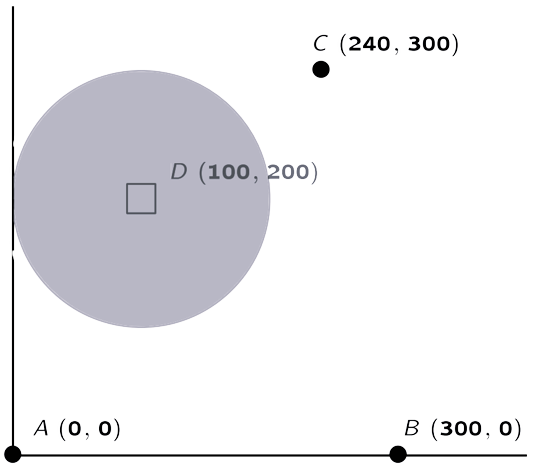
\includegraphics[width=0.4\linewidth]{images/example3.png}
        \end{figure}
        The cost of the pipelines is proportional to the square of their length.
        The refinery must be at least 100 km away from point $D=(100,200)$.
        The objective is to find the location for the refinery that minimizes the total pipeline cost.

        The mathematical model for this problem can be defined as follows:
        \begin{itemize}
            \item Decision variables: the coordinates of the refinery, denoted as $x_1,x_2$. 
            \item Objective function: we need to minimize the total pipeline cost, which is the sum of the squared distances between the oil pits and the refinery:
            \begin{align*}
                \min{z} &=\left[ (x_1-0)^2+(x_2-0)^2 \right] \\
                        &+ \left[ (x_1-300)^2+(x_2-0)^2 \right] \\
                        &+ \left[ (x_1-240)^2+(x_2-300)^2 \right] 
            \end{align*}
            \item Constraints: there is a constraint that ensures the refinery is at least 100 km away from point $D=(100,200)$. 
                The constraint can be represented as:
                \[\sqrt{{\left( x_1-100 \right)}^2+{\left( x_2-100 \right)}^2} \geq 100\]
            \item Variable type: $x_1,x_2 \in \mathbb{R}$
        \end{itemize}
    \end{example}

    \section{Mathematical programming problem}
    \begin{table}[H]
        \centering
        \begin{tabular}{c|ccc|}
        \cline{2-4}
                                                                   & \textbf{Decisions} & \textbf{Objective} & \textbf{Uncertainty} \\ \hline
        \multicolumn{1}{|c|}{\textit{Mathematical programming}}    & single                   & one                          & no                   \\
        \multicolumn{1}{|c|}{\textit{Multi-objective programming}} & single                   & multiple                     & no                   \\
        \multicolumn{1}{|c|}{\textit{Stochastic programming}}      & -                        & -                            & yes                  \\
        \multicolumn{1}{|c|}{\textit{Game theory}}                 & multiple                 & -                            & no                   \\ \hline
        \end{tabular}
    \end{table}
    We will delve into the realm of mathematical programming problems, where the primary aim typically revolves around minimizing or maximizing a specified function. 
    Notably, it's worth mentioning that the maximization of a function $f(x)$ is essentially equivalent to the minimization of $-f(x)$. 
    These problems are defined by the following characteristics:
    \begin{itemize}
        \item Decision variables $x \in \mathbb{R}^n$: these are numerical variables that serve as identifiers for potential solutions.
        \item Feasible region $X \subseteq \mathbb{R}^n$: this is the set of admissible values for the decision variables.
        \item Objective function $f:X \rightarrow\mathbb{R}$: this function quantitatively expresses the value of each feasible solution.
    \end{itemize}
    The core objective in solving a mathematical programming problem is to uncover a feasible solution that is globally optimal. 
    In some cases, the problem may prove to be infeasible, unbounded, possess a unique optimal solution, or offer a multitude of optimal solutions. 
    When dealing with particularly challenging problems, it may be necessary to settle for a feasible solution that represents a local optimum.
    
    Mathematical programming can be categorized into the following classes:
    \begin{enumerate}
        \item Linear Programming.
        \item Integer Linear Programming.
        \item Nonlinear Programming. 
    \end{enumerate}
    
    \subsection{Multi-objective programming}
    Multi-objective programming can be approached in various ways. 
    Suppose our goal is to minimize $f_1(x)$ while simultaneously maximizing $f_2(x)$. 
    In this context, we can:
    \begin{enumerate}
        \item Combine the objectives into a single objective problem by representing both objectives in the same units. 
            This involves minimizing a weighted combination of the objectives, as follows:
            \[\min{\lambda_1f_1(x)-\lambda_2f_2(x)}\]
            with appropriate scalar values $\lambda_1$ and $\lambda_2$.
        \item Prioritize the primary objective and transform the other objective into a constraint. 
            In this approach, the focus is on optimizing the primary objective function while ensuring that the secondary objective satisfies a specified constraint. 
            This is achieved as follows:
            \[\max_{x \in X}f_2(x) \:\:\:\: f_1(x)\leq \varepsilon\]
            with an appropriate constant value $\varepsilon$. 
    \end{enumerate}

\newpage

\chapter{Algorithms}
    \section{Complexity}
    \begin{definition}
        An \emph{algorithm} is a step-by-step sequence of instructions designed to solve any given instance of a problem.

        An \emph{instance}, denoted as $I$, pertaining to a problem $P$, is a specific and unique case derived from the problem $P$.
    \end{definition}

    The runtime of an algorithm is contingent on both the specific instance and the computer it runs on. 
    To assess the algorithm's complexity while abstracting from hardware variations, we focus on evaluating its performance as a function of the instance's size, independently of the underlying hardware. 
    For this purpose, we consider the count of elementary operations, presuming that each operation carries an equivalent cost. 
    Since determining the precise count of elementary operations is often a formidable task, we resort to considering the asymptotic count of elementary operations in the worst-case scenario.
    \begin{definition}
        A function $f$ is denoted as being \emph{order of} $g$ and expressed as:
        \[f(n)=O(g(n))\]
        If there exists a positive constant $c$ such that $f(n)$ is less than or equal to $c \cdot g(n)$ for sufficiently large values of $n$.
    \end{definition}
    We can categorize algorithms into two primary classes based on their worst-case complexity:
    \begin{itemize}
        \item Polynomial: characterized by a complexity of $O(n^d)$, where $d$ is a constant.
        \item Exponential: demonstrating a complexity of $O(2^n)$. 
    \end{itemize}
    Algorithms with a high-order polynomial complexity are generally considered inefficient in practical applications.
    \begin{figure}[H]
        \centering
        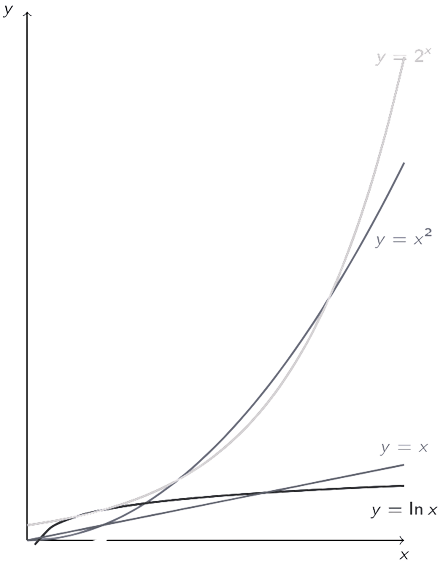
\includegraphics[width=0.25\linewidth]{images/complexity.png}
        \caption{Plot of various algorithm's complexity}
    \end{figure}
    \begin{definition}
        The size of an instance denoted as $\left\lvert I \right\rvert$ represents the number of bits required to represent that instance.

        A problem $P$ is considered \emph{polynomially solvable} if there exists a polynomial time algorithm that can provide an optimal solution for any given instance.
    \end{definition}
    For many discrete optimization problems, the most efficient algorithm available today demands a number of elementary operations that, in the worst-case scenario, grows exponentially with the size of the instance.
    \begin{definition}
        \emph{$\mathcal{NP}$-hard computational problems} are, at the very least, as challenging as a broad spectrum of exceptionally difficult problems for which no polynomial time algorithm has been identified to date.
    \end{definition}
    The $\mathcal{N}\mathcal{P}$-hardness of a problem is a very strong evidence that is inherently difficult. 
    However, this doesn't imply that it cannot potentially be solved using a polynomial time algorithm.

    \section{Definitions}
    \begin{definition}
        An algorithm is considered \emph{exact} when it is capable of delivering an optimal solution for every single instance.

        In contrast, an algorithm is deemed \emph{heuristic} when it is not guaranteed to provide an optimal solution for all instances.

        A \emph{greedy algorithm} progressively builds a feasible solution by consistently making locally optimal choices at each step, without revisiting or reevaluating prior selections.
    \end{definition}

    \section{Dynamic programming}
    Dynamic programming, introduced by Richard Bellman in 1953, is a versatile method employed to find optimal solutions consisting of a sequence of elementary decisions.
    This is achieved by resolving a series of recursive equations.

    Dynamic programming is well-suited for a wide range of sequential decision problems as long as they adhere to the optimality property.
    
    In contemporary applications, dynamic programming finds utility across various domains, including optimal control, equipment maintenance and replacement, and the selection of inspection points along a production line.

\newpage

\chapter{Network optimization models}
    \section{Introduction}
    Numerous decision-making problems find their representation in the realm of graphs.
    \begin{definition}
        A graph is described as a pair $G=(N,E)$, comprising a set of nodes denoted as $N$ and a set of edges or arcs $E$, where these edges link the nodes in pairs.

        In the case of an undirected graph, an edge connecting nodes $i$ and $j$ is denoted as ${i,j}$, while in a directed graph, it is represented as $(i,j)$.    
    \end{definition}
    \begin{example}
        Consider a road network connecting a total of "n" cities, which can be effectively represented by a graph. 
        In this representation, each city corresponds to a node, and the connections between them are represented as edges.        
        \begin{figure}[H]
            \centering
            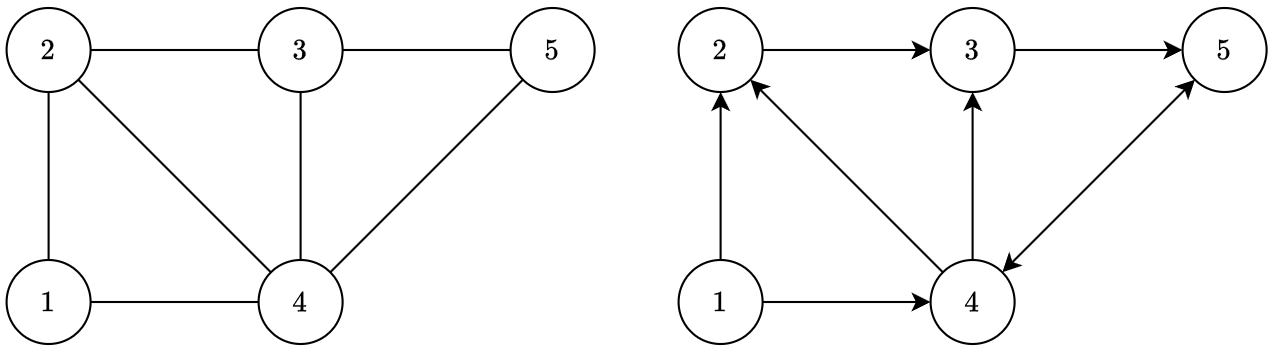
\includegraphics[width=0.75\linewidth]{images/graph.png}
        \end{figure}
        The left graph is undirected and defined as follows:
        \begin{itemize}
            \item $N=\{1,2,3,4,5\}$
            \item $E=\{\{1,2\},\{1,4\},\{2,3\},\{2,4\},\{3,4\},\{3,5\},\{4,5\}\}$
        \end{itemize}
        The right graph is directed and defined as:
        \begin{itemize}
            \item $N=\{1,2,3,4,5\}$
            \item $E^{'}=\{(1,2),(1,4),(2,3),(2,4),(3,4),(3,5),(4,5)\}$
        \end{itemize}
    \end{example}
    \newpage
    \begin{definition}
        Nodes are considered \emph{adjacent} when they are linked by an edge.
        
        An edge labeled as $e$ is deemed \emph{incident} to a node $v$ when node $v$ serves as one of the endpoints of the edge $e$.
        
        In undirected graphs, the \emph{degree of a node} signifies the count of edges incident to that particular node. 
        
        In directed graphs, the \emph{in-degree of a node} represents the number of arcs that have it as their successor, while the \emph{out-degree of a node} denotes the quantity of arcs that have it as their predecessor.
    \end{definition}
    \begin{example}
        In the undirected graph, we observe that nodes 1 and 2 are adjacent, while node 1 and node 3 are not. 
        The edge $\{1,2\}$ is incident to nodes 1 and 2. 
        Node 1 has a degree of 2, and node 4 has a degree of 4.
        In the directed graph, node 1 exhibits an in-degree of 0 and an out-degree of 2.
        \begin{figure}[H]
            \centering
            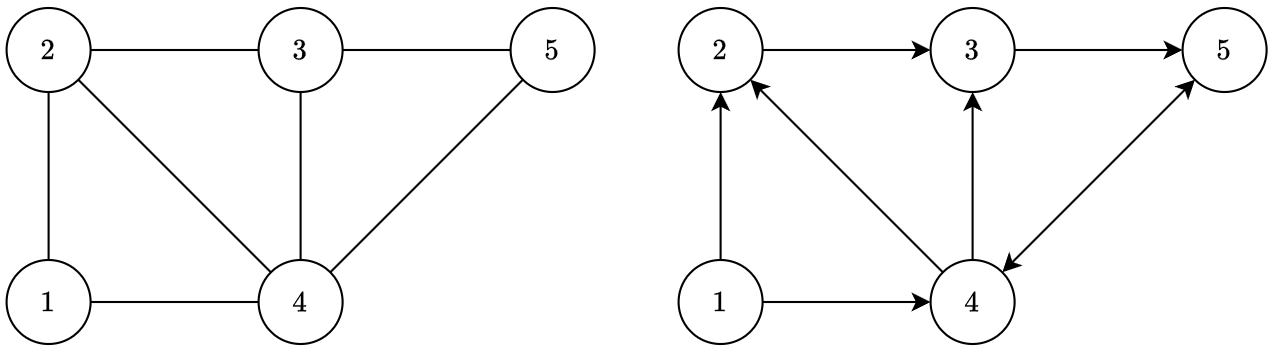
\includegraphics[width=0.75\linewidth]{images/graph.png}
        \end{figure}
    \end{example}
    \begin{definition}
        A \emph{directed path from $i \in N$ to $j \in N$} is a sequence $p=\langle \{v_1,v_2\},\{v_2,v_3\},\dots,\{v_{k-1},v_k\}\rangle $ connecting nodes $v_1$ and $v_k$.

        Nodes $u$ and $v$ are \emph{connected} if there is a path connecting them. 
        A graph $(N,E)$ is connected if $u,v$ are connected for any $u,v \in N$. 
        
        A graph is \emph{strongly connected} if $u$ and $v$ are connected by a directed path for any $u,v \in N$. 
        
        A \emph{cycle} or circuit is a path with $v_1=v_k$.
    \end{definition}
    \begin{example}
        The undirected graph has a path $\langle \{2,3\},\{3,4\},\{4,5\}\rangle$ connecting node $2$ to node $5$, thus indicating a connection between these nodes.
        
        The directed graph has a directed path $\langle (3,5),(5,4),(4,2),(2,3),(3,4) \rangle$ from node $3$ to node $4$. So we say those nodes are not strongly connected. 
        
        In the undirected graph, we observe a cycle $\langle \{2,3\},\{3,5\},\{5,4\},\{4,2\}\rangle$. 
        In the directed graph, a circuit is present, specifically $\langle (2,3),(3,4),(4,2) \rangle$. 
        \begin{figure}[H]
            \centering
            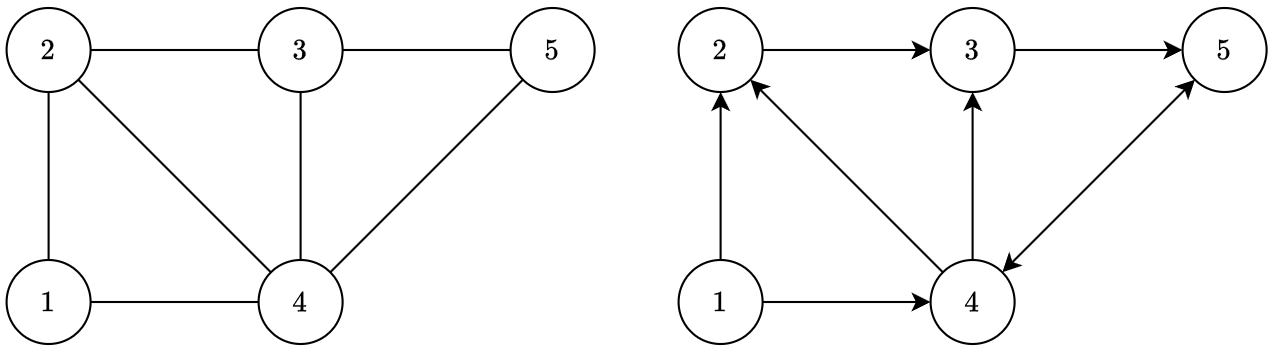
\includegraphics[width=0.75\linewidth]{images/graph.png}
        \end{figure}
    \end{example}
    \newpage
    \begin{definition}
        A graph is \emph{bipartite} if there is a partition $N=N_1 \cup N_2$ with $N_1 \cap N_1 = \varnothing$ such that no edge connects nodes in the same subset. 

        A graph is \emph{complete} if $E=\{ \{v_i,v_j\} | v_i,v_j \in N \land i \leq j \}$
    \end{definition}
    \begin{example}
        The graphic on the left is bipartite because we can find two subsets of nodes such that $N=N_1 \cup N_2$ with $N_1 \cap N_1 = \varnothing$ that are: $N_1=\{1,2,3\}$ and $N_2=\{4,5\}$. 
        The graph on the right is a complete graph because all the nodes are connected with each other. 
        \begin{figure}[H]
            \centering
            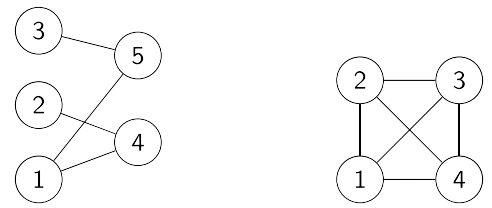
\includegraphics[width=0.5\linewidth]{images/bipcomp.png}
        \end{figure}
    \end{example}
    \begin{definition}
        Given a directed graph $G=(N,A)$ and $S \subset NM$, the \emph{outgoing cut} induced by $S$ is:
        \[ \delta^{+}(S)=\{(u,v) \in A | u \in S \land v \in N-S \} \]

        Given a directed graph $G=(N,A)$ and $S \subset NM$, the \emph{incoming cut} induced by $S$ is:
        \[ \delta^{-}(S)=\{(u,v) \in A | v \in S \land u \in N-S \} \]
    \end{definition}
    \begin{example}
        In the graph presented below, we can observe that:
        \begin{itemize}
            \item $\delta^{+}(\{1,4\})=\{(1,2),(4,2),(4,5)\}$
            \item $\delta^{-}(\{1,4\})=\{(3,4),(5,4)\}$
        \end{itemize}
        \begin{figure}[H]
            \centering
            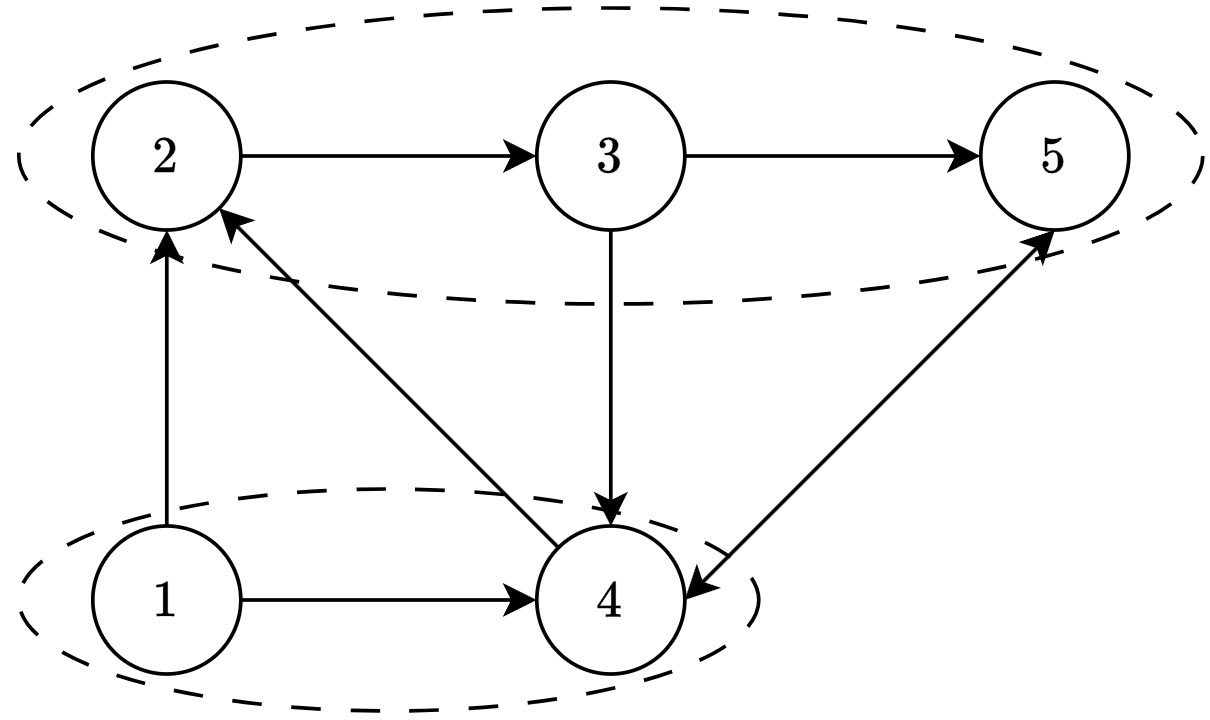
\includegraphics[width=0.75\linewidth]{images/cuts.png}
        \end{figure}
    \end{example}
    An undirected graph with $n$ nodes has at most $m=n(n-1)$ arcs. 
    A directed graph with $n$ nodes has at most $m=\dfrac{n(n-1)}{2}$ arcs.
    \newpage
    \begin{definition}
        For a given graph with $m$ representing the number of arcs or edges and $n$ representing the number of nodes, we classify a graph as \emph{dense} when:
        \[m \approx n^2\]

        Conversely, for the same graph, it is considered \emph{sparse} when:
        \[m \ll n^2\]
    \end{definition}
    The most suitable method for representing a dense graph is by utilizing an $n \times n$ adjacency matrix, defined as follows:
    \[
    \begin{cases}
        a_{ij}=1 \:\:\:\:\:\: \textnormal{if }(i,j) \in A \\
        a_{ij}=0 \:\:\:\:\:\: \textnormal{otherwise}    
    \end{cases}    
    \]
    Conversely, for a sparse graph, the most effective approach is to use lists of successors for each node.
    \begin{example}
        The adjacency matrix for the depicted graph is as follows:
        \[A=\begin{bmatrix}
            0 & 1 & 0 & 1 & 0 \\
            0 & 0 & 1 & 0 & 0 \\
            0 & 0 & 0 & 1 & 1 \\
            0 & 1 & 0 & 0 & 1 \\
            0 & 0 & 0 & 1 & 0 
            \end{bmatrix}\]
        Furthermore, the list of successors is presented as follows:
        \[S(1)=\{2,4\} \:\:\: S(2)=\{3\} \:\:\:S(3)=\{4,5\} \:\:\: S(4)=\{2,5\} \:\:\: S(5)=\{4\} \:\:\:\]
        \begin{figure}[H]
            \centering
            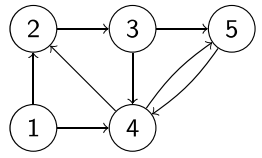
\includegraphics[width=0.3\linewidth]{images/graphs.png}
        \end{figure}
    \end{example}
    \begin{definition}
        $G^{'}=(N^{'},E^{'})$ is a \emph{sub-graph} of $G=(N,E)$ if $N^{'} \subseteq N$ and $E^{'} \subseteq E$. 

        A \emph{tree} $G_T=(N^{'},T)$ \emph{of $G$} is a connected and acyclic sub-graph of $G$. 

        $G_T=(N^{'},T)$ is a \emph{spanning tree of $G$} if it contains all nodes in $G$. 

        The \emph{leaves} of a tree are the nodes of degree one. 
    \end{definition}
    \begin{example}G
        Considering the provided graph:
        \begin{figure}[H]
            \centering
            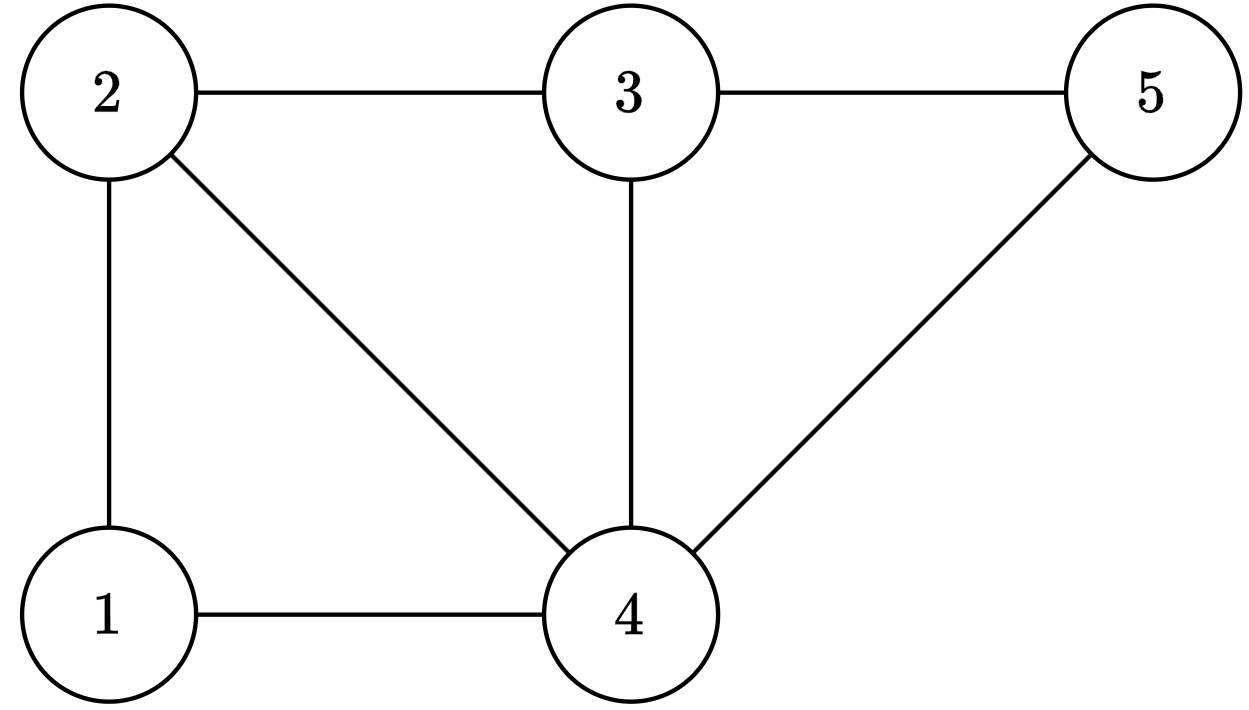
\includegraphics[width=0.3\linewidth]{images/sgraph.png}
        \end{figure}
        We can identify three different structures: a sub-graph, a tree, and a spanning tree. 
        These structures are visually depicted in the modified graph below:
        \begin{figure}[H]
            \centering
            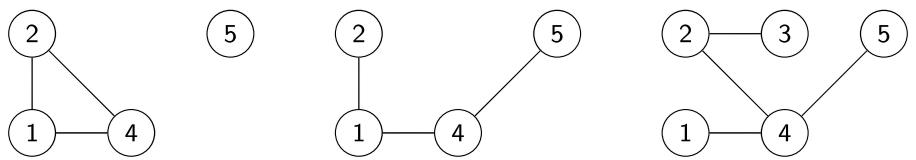
\includegraphics[width=0.8\linewidth]{images/sgraphmod.png}
        \end{figure}
    \end{example}
    \begin{property}
        Every tree with $n$ nodes has $n-1$ edges. 
    \end{property}
    \begin{proof}
        We will demonstrate this property with a proof by induction. 
        For the base case we have that the claim holds for $n=1$. 
        For the inductive step we have to show that, if this is true for trees with $n$ nodes, then it is also true for those with $n+1$ nodes. 
        Let $T_1$ be a tree with $n+1$ nodes and recall that any tree with $n \geq 2$ nodes has at least two leaves. 
        By deleting one of the leaf and its incident edge we obtain a tree $T_2$ with $n$ nodes. 
        By induction hypothesis, $T_2$ has $n-1$ edges. 
        Therefore, the tree $T_1$ has $n-1+1=n$ edges. 
    \end{proof}
    \begin{property}
        Any pair of nodes in a tree is connected via a unique path. 
    \end{property}
    \begin{property}
        By adding a new edge to a tree, we create a unique cycle. 
    \end{property}
    \begin{property}
        Let $G_T=(N,T)$ be a spanning tree of $G=(N,E)$. 
        Consider an edge $e \notin T$ and the unique cycle $C$ of $T \cup \{e\}$. 
        For each edge $f \in C-\{e\}$, the sub-graph $T\cup \{e\}-\{f\}$ is also a spanning tree of $G$. 
    \end{property}

    \section{Graph reachability problem}
    In a directed graph $G=(N,A)$, given a specific node $s$, find all the nodes that can be reached starting from node $s$.
    \begin{algorithm}[H]
        \caption{Graph reachability problem}
            \begin{algorithmic}[1]
                \State $Q \leftarrow \{s\}$
                \State $M \leftarrow \{\varnothing\}$
                \While {$Q \neq 0$}
                    \State $u \leftarrow \textnormal{node in } Q$
                    \State $Q \leftarrow Q-\{u\}$
                    \State $M \leftarrow M \cup \{u\}$
                    \For {$(u,v) \in \delta^{+}(u)$}
                        \If {$v \notin M$ and $v \notin Q$}
                            \State $Q \leftarrow Q \cup \{v\}$
                        \EndIf
                    \EndFor
                \EndWhile
            \end{algorithmic}
    \end{algorithm}
    The algorithm's worst-case time complexity is $O(n^2)$. 
    \begin{example}
        Given the graph and the starting node $s=2$, the algorithm proceeds through the following steps:
        \begin{enumerate}
            \item $Q=\{2\} \:\:\:\:\:\:\:\:\:\:\: M=\varnothing$
            \item $Q=\{3\} \:\:\:\:\:\:\:\:\:\:\: M=\{2\}$
            \item $Q=\{4,5\} \:\:\:\:\:\:\: M=\{2,3\}$
            \item $Q=\{5\} \:\:\:\:\:\:\:\:\:\:\: M=\{2,3,4\}$
            \item $Q=\varnothing \:\:\:\:\:\:\:\:\:\:\:\:\:\: M=\{2,3,4,5\}$
        \end{enumerate}
        As a result, nodes $\{2,3,4,5\}$ are determined to be reachable from node two.
        \begin{figure}[H]
            \centering
            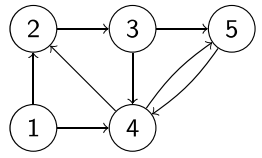
\includegraphics[width=0.3\linewidth]{images/graphs.png}
        \end{figure}
    \end{example}

    \section{Minimum spanning tree problem}
    Given an undirected graph $G=(N,E)$ and a cost function, find a spanning tree $G_T=(N,T)$ of minimum total cost: 
    \[\min_{T \in X} \sum_{e \in T}c_e\]
    Here, $X$ is the set of all spanning trees of $G$. 
    \begin{theorem}
        A complete graph with $n$ nodes $(n \geq 1)$ has $n^{(n-2)}$ spanning trees. 
    \end{theorem}
    To determine the spanning tree with the lowest total cost, we can employ an algorithm that incrementally constructs the spanning tree. 
    The algorithm's fundamental concept is:
    \begin{enumerate}
        \item Start by choosing any node arbitrarily and establish a connection to the nearest distinct node.
        \item Locate an unconnected node that is nearest to a connected node, and proceed to connect these two nodes. 
            Continue this process until all nodes are connected.
    \end{enumerate}
    \begin{example}
        Let's apply Prim's algorithm to the following graph:
        \begin{figure}[H]
            \centering
            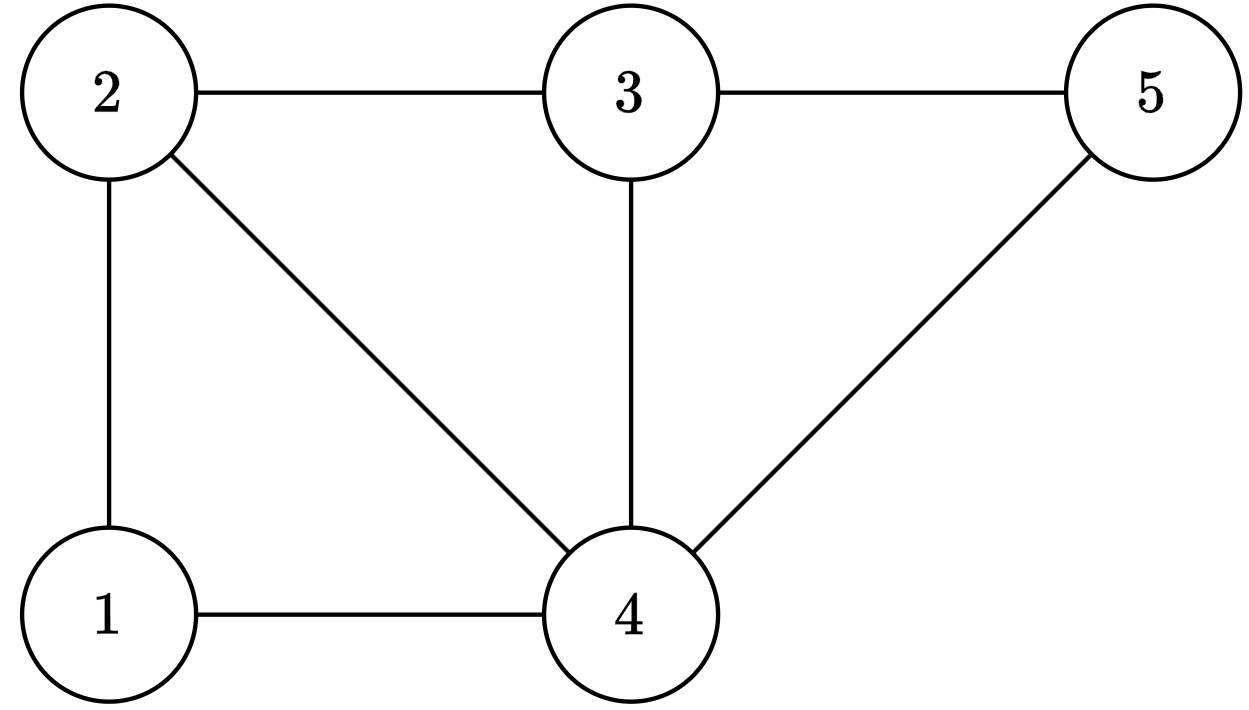
\includegraphics[width=0.3\linewidth]{images/sgraph.png}
        \end{figure}
        We start by selecting node 3 as our initial node. 
        Therefore, we have two sets: 
        \begin{itemize}
            \item $S=\{3\}$.
            \item $T=\{\varnothing\}$.
        \end{itemize}
        Next, we follow these steps:
        \begin{itemize}
            \item The edge with the minimum cost connects nodes 3 and 4. 
                Now we have: 
                \begin{itemize}
                    \item $S=\{3,4\}$.
                    \item $T=\{\{3,4\}\}$.
                \end{itemize}
            \item The edge with the minimum cost connects nodes 1 and 4. 
                Now we have:
                \begin{itemize}
                    \item $S=\{1,3,4\}$. 
                    \item $T=\{\{3,4\},\{1,4\}\}$.
                \end{itemize}
            \item The edge with the minimum cost connects nodes 4 and 5. 
            Now we have: 
            \begin{itemize}
                \item $S=\{1,3,4,5\}$.
                \item $T=\{\{3,4\},\{1,4\},\{4,5\}\}$.
            \end{itemize}
            \item The edge with the minimum cost connects nodes 4 and 5. 
            Now we have:
            \begin{itemize}
                \item $S=N$.
                \item $T=\{\{3,4\},\{1,4\},\{4,5\},\{2,4\}\}$.
            \end{itemize}
        \end{itemize}
        In this case, the total cost is equal to $c(T)=6$. 
        Graphically, the resulting minimum spanning tree is as shown below:
        \begin{figure}[H]
            \centering
            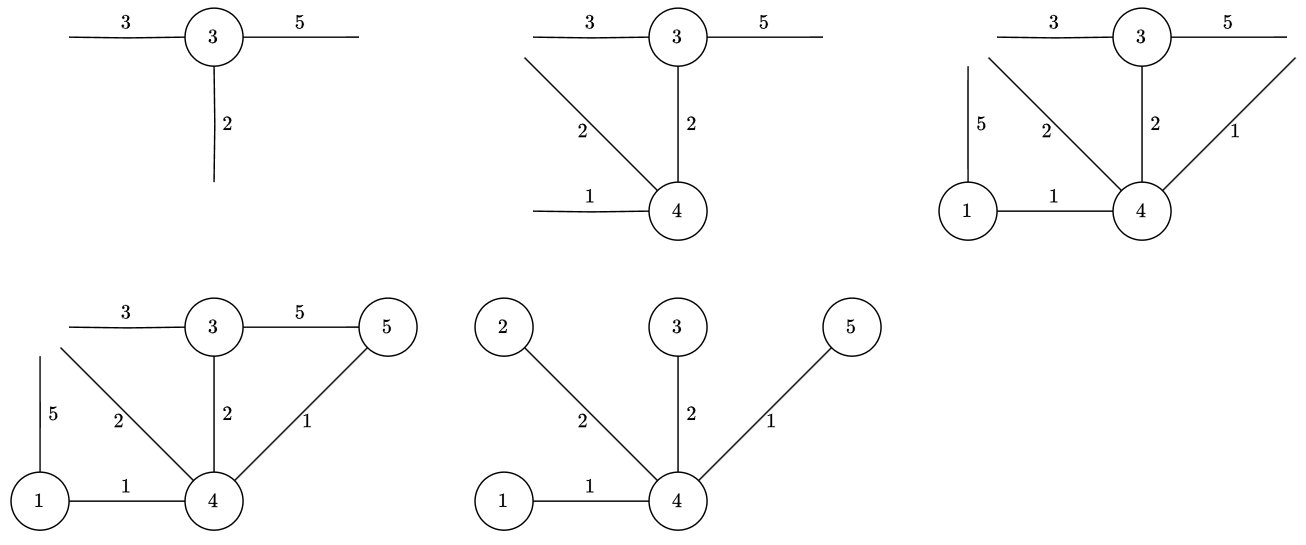
\includegraphics[width=0.75\linewidth]{images/MST.png}
        \end{figure}
    \end{example}
    \begin{algorithm}[H]
        \caption{Prim's algorithm for the minimum cost spanning tree problem}
            \begin{algorithmic}[1]
                \State $S \leftarrow \{u\}$
                \State $T \leftarrow \{\varnothing\}$
                \While {$\left\lvert T \right\rvert < n-1$}
                    \State $\{u,v\}\leftarrow \textnormal{edge in } \delta(S) \textnormal{ of minimum cost}$
                    \State $S \leftarrow S \cup \{v\}$
                    \State $T \leftarrow T \cup \{u,v\}$
                \EndWhile
            \end{algorithmic}
    \end{algorithm}
    Where $u \in S$ and $v \in N-S$. 
    The worst-case complexity is $O(n^2)$. 
    \newpage
    \begin{proposition}
        Prim's algorithm is exact. 
    \end{proposition}        
    The exactness does not depend on the choice of the first node nor on the selected edge of minimum cost in $\delta(S)$. 
    \begin{property}
        Let $F$ be a partial tree contained in an optimal tree of $G$. 
        Consider $e\{u,v\}\in \delta(S)$ of minimum cost, then there exists a minimum cost spanning tree of $G$ containing $e$. 
    \end{property}
    \begin{proof}
        By contradiction, assume $T^{} \subseteq E$ is a minimum cost spanning tree with $F \subseteq T^{}$ and $e \notin T^{}$. 
        Adding edge $e$ to $T^{}$ creates the cycle $C$. 
        Let $f \in \delta(S) \cap C$: 
        \begin{itemize}
            \item If $c_e=c_f$, then $T^{}\cup\{e\}-\{f\}$ is also optimal since it has same cost of $T^{}$.
            \item If $c_e<c_f$, then $c\left(T^{}\cup\{e\}-\{f\}\right)<C(T^{})$, hence $T^{*}$ is not optimal.
        \end{itemize}
    \end{proof}
    \begin{proposition}
        Prim's algorithm is greedy. 
    \end{proposition}     
    At each step a minimum cost edge is selected among those in the cut $\delta (S)$ induced by the current set of nodes $S$. 
    \begin{definition}
        Given a spanning tree $T$, an edge $e \notin T$ is \emph{cost decreasing} if when $e$ is added to $T$ it creates a cycle $C$ with $C \subseteq T \cup \{e\}$ and $\exists f \in C-\{e\}$ such that $c_e<c_f$. 
    \end{definition}
    \begin{example}
        In the context of the given graph:
        \begin{figure}[H]
            \centering
            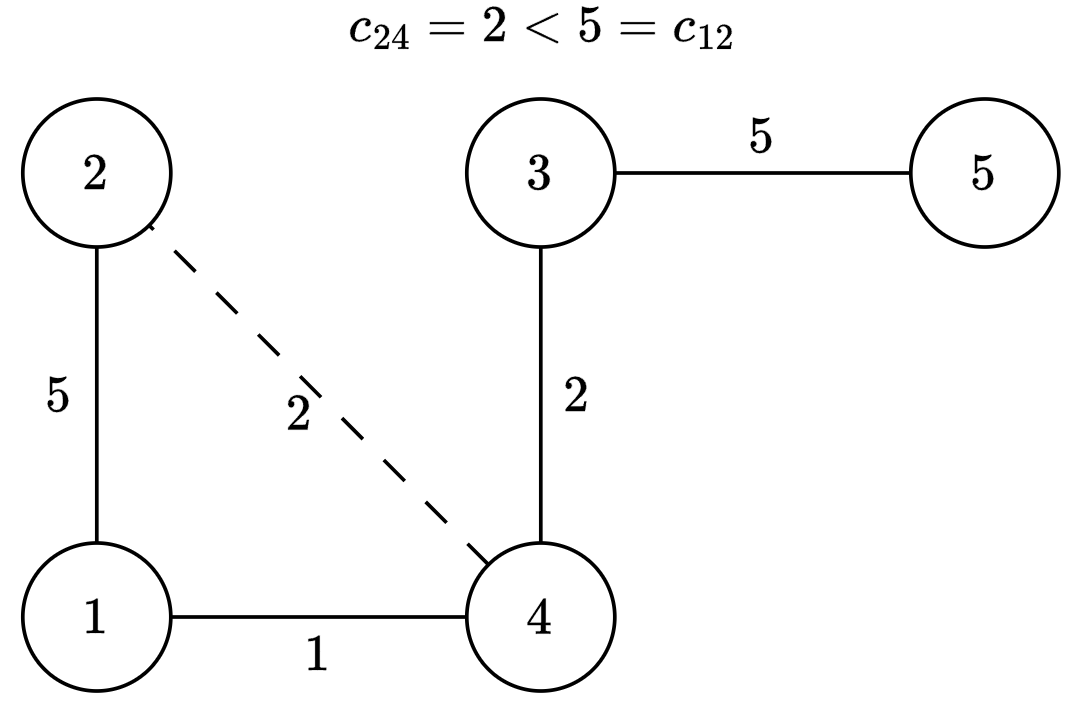
\includegraphics[width=0.5\linewidth]{images/costdecreasing.png}
        \end{figure}
        Since we have the equation:
        \[c(T \cup \{e\}-\{f\})=c(T)+c_e-c_f\]
        If edge $e$ is cost decreasing, it implies that:
        \[c(T \cup \{e\}-\{f\})<c(T)\]
    \end{example}
    \begin{theorem}
        A tree $T$ is of minimum total cost if and only if no cost decreasing edge exists. 
    \end{theorem}
    \begin{proof}[of direct implication]
        If a cost-decreasing edge exists, then $T$ is not of minimum total cost.
    \end{proof}
    \begin{proof}[of inverse implication]
        When there are no cost-decreasing edges, it implies that the spanning tree $T$ has the minimum total cost.
        Consider a minimum-cost spanning tree denoted as $T^{*}$, which is obtained through Prim's algorithm.
        It is possible to confirm that, by gradually exchanging one edge at a time, $T^{*}$ can be transformed step by step into $T$ without altering the overall cost.
        Consequently, we can conclude that $T$ is also an optimal solution.
    \end{proof}
    The optimality condition provides a means to confirm the optimality of a spanning tree $T$. 
    To determine if $T$ is optimal, it is sufficient to examine whether each edge $e$ in the set $E-T$ is not a cost-decreasing edge.

    \section{Graph shortest path problem}
    \subsection{Dijkstra's algorithm}
    Given a directed graph $G=(N,A)$ with a cost $c_j \in R$ for each arc $(i,j) \in A$, and two nodes $s$ and $t$, determine a minimum cost path from $s$ to $t$. 

    Each value $c_j$ represents the cost associated with arc $(i,j) \in A$. 
    Here, node $s$ is designated as the source or origin, while node $t$ is specified as the destination or sink.
    \begin{definition}
        A path is considered \emph{simple} when it ensures that each node is visited exactly once, without any repetitions.
    \end{definition}
    \begin{property}
        If $c_j \geq 0$ for all $(i,j) \in A$, there is at least one shortest path which is simple. 
    \end{property}
    Dijkstra's algorithm takes as input a graph $G = (N, A)$ with non-negative arc costs and a designated starting node $s$. 
    The primary purpose of this algorithm is to determine the shortest paths from $s$ to all other nodes within $G$.
    The algorithm's core principle involves systematically processing nodes based on their increasing order of the cost of the shortest path from s to each of them. 
    For each node $j$ belonging to $N$, we assign two labels:
    \begin{itemize}
        \item $L_j$, which represents the cost of the minimum-cost path from s to j.
        \item $pred_j$, which identifies the predecessor of $j$ along the shortest path from $s$ to $j$.
    \end{itemize} 
    It is important to note that Dijkstra's algorithm follows a greedy approach with respect to path from $s$ to $j$. 
    \begin{example}
        Let's apply Dijkstra's algorithm to a given graph, starting with node 1 as the initial node. 
        We assign labels as follows:
        \begin{figure}[H]
            \centering
            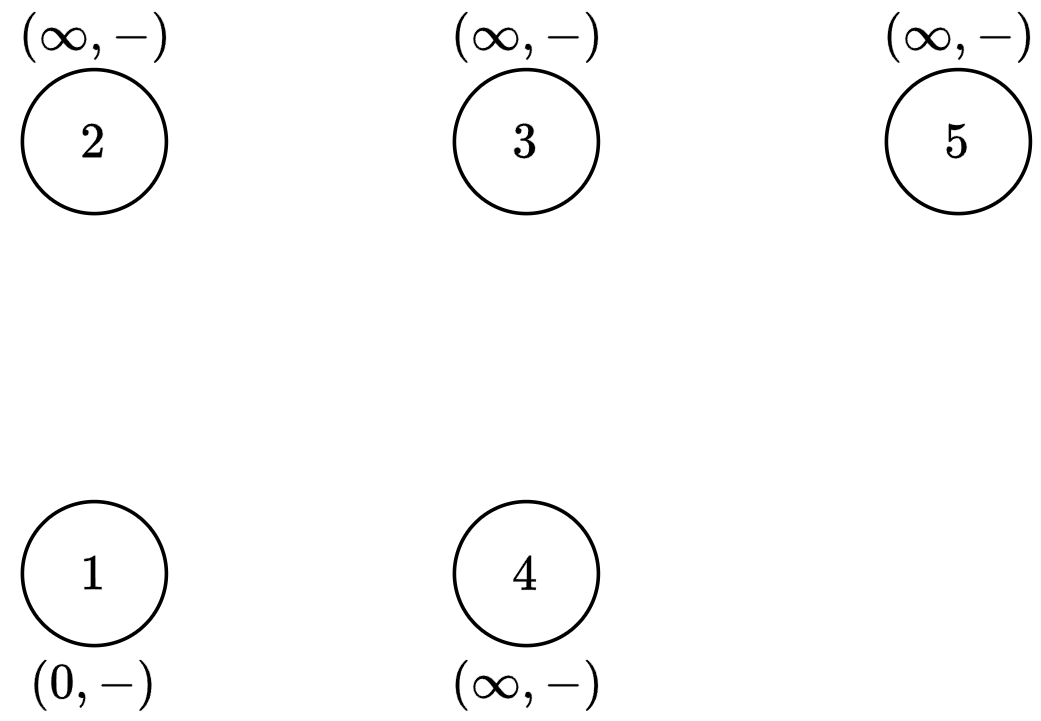
\includegraphics[width=0.2\linewidth]{images/D1.png}
        \end{figure}
        Next, we examine all arcs leading from the starting node to other nodes and update their labels:
        \begin{figure}[H]
            \centering
            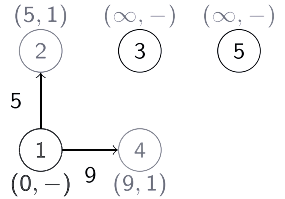
\includegraphics[width=0.2\linewidth]{images/D2.png}
        \end{figure}
        Moving to node 2, we explore reachable nodes. 
        In this case, we find the shortest path from the initial node to 4, so we update the label for 4:
        \begin{figure}[H]
            \centering
            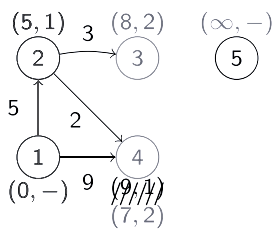
\includegraphics[width=0.2\linewidth]{images/D3.png}
        \end{figure}
        Now, we proceed to node 4, which is the closest node to the starting point.
         We check all arcs leading to other nodes:
        \begin{figure}[H]
            \centering
            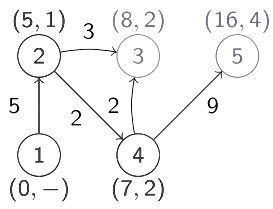
\includegraphics[width=0.2\linewidth]{images/D4.png}
        \end{figure}
        We repeat this process for the remaining nodes, considering them in ascending order of cost from the start:
        \begin{figure}[H]
            \centering
            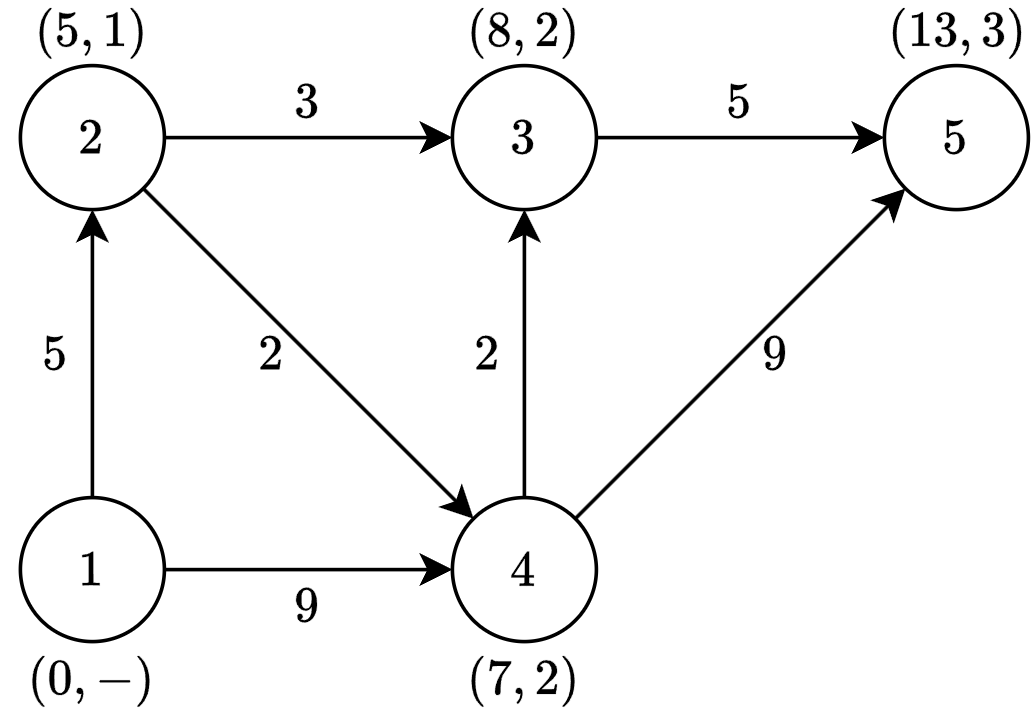
\includegraphics[width=0.4\linewidth]{images/D5.png}
        \end{figure}
        At this point, we can trace back the shortest path to any node in the graph using the predecessor label. 
        For instance, the shortest path from $s$ to 5 has a cost of 13, and the path is $(1,2,3,5)$. 
    \end{example}

    The inputs to the algorithm consist of a graph $G=(N, E)$ with non-negative costs assigned to its arcs, and a designated starting node $s$, which is a member of $N$.
    \begin{algorithm}[H]
        \caption{Dijkstra's algorithm for the graph shortest path problem}
            \begin{algorithmic}[1]
                \State $S \leftarrow \varnothing$
                \State $X \leftarrow \{s\}$
                \For {$u \in N$}
                    \State $L_u \leftarrow +\infty$
                \EndFor
                \State $L_s \leftarrow 0$
                \While {$\left\lvert S \right\rvert \neq n$}
                    \State $u \leftarrow \textnormal{argmin}\{L_i|i \in X\}$
                    \State $X \leftarrow X-\{u\}$
                    \State $S \leftarrow S \cup \{u\}$
                    \For {$(u,v) \in \delta^{+}(u) \: \textnormal{such that} \: L_v> L_u + c_{uv} $}
                        \State $L_v \leftarrow L_u+c_{uv}$
                        \State $pred_v \leftarrow u$
                        \State $X \leftarrow X \cup \{v\}$
                    \EndFor
                \EndWhile
            \end{algorithmic}
    \end{algorithm}
    The worst-case time complexity of this algorithm is $O(n^3)$. 
    \begin{proposition}
        Dijkstra's algorithm is exact. 
    \end{proposition}
    \begin{proof}
        At the $k$-th step: $S = \{s,i_2,\dots,i_k\}$ and 
        \[L_j=
        \begin{cases}
            \textnormal{cost of a minimum path from } s \textnormal{ to } j,\:j \in S \\ 
            \textnormal{cost of a minimum path with all intermediate nodes in } S, \: j \notin S
        \end{cases}
        \]
        By induction on the number $k$ of steps: 
        \begin{itemize}
            \item Base case: it is easy to see that the statement holds for $k = 1$, since 
                \[S=\{s\},\: L_s=0,\: L_j= +\infty,\: \forall j \neq S \]
            \item Inductive step: we must prove that, if the statement holds at the $k$-th step, it must also hold for the $(k + 1)$-th step. 
        \end{itemize}
        In the $(k + 1)$-th step let $u \notin S$be the node that is inserted in $S$ and $\varnothing$ the path from $s$ to $u$ such that:
        \[L_v + c_{uv} \leq L_i + C_{ij},\: \forall(i,j) \in \delta^{+}(S)\]
        Let us verify that every path $\pi$ from $s$ to $u$ has $c(\pi) \geq c(\varnothing)$. There exist $i \in S$ and $j \notin S$ such that: 
        \[\pi= \pi_1 \cup \{(i,j)\} \cup \pi_2\]
        Where $(i, j)$ is the first arc in $\pi \cap \delta^{+}(S)$. Moreover: 
        \[c(\pi) = c(\pi_1) + c_{ij} + c(\pi_2) \geq L_i + c_{ij}\]
        Because $c_{ij} \geq 0$, thus, $c(\pi_2) \geq 0$, and by the induction assumption, $c(\pi_1) \geq L_i$. Finally, by the choice of $(v,u)$ we have: 
        \[L_i + c_{ij} \geq L_v + c_{vu} = c(\varnothing)\]
    \end{proof}
    We can observe the following points:
    \begin{itemize}
        \item A collection of the shortest paths from the starting node $s$ to all nodes $j$ can be obtained using the predecessor vector.
        \item The union of a set of the shortest paths from node $s$ to all the other nodes of $G$ is the shortest path trees rooted at $s$. 
            These shortest path trees are distinct from minimum-cost spanning trees.
        \item Dijkstra's algorithm is not applicable when there are arcs with negative costs.
    \end{itemize}

    \subsection{Floyd-Warshall's algorithm}
    When the graph $G$ contains a negative-cost cycle, the well-defined nature of the shortest path problem is compromised. 
    Such cycles repeatedly lead to a decrease in cost, making it impossible to identify a finite shortest path from node $s$ to $t$.
    To address this issue, the Floyd-Warshall algorithm is employed, as it is capable of detecting negative-cost cycles.
    The Floyd-Warshall algorithm provides a comprehensive set of shortest paths between all pairs of nodes, even in the presence of arcs with negative costs. 
    This algorithm is founded on an iterative process known as a triangular operation.
    It employs $n \times n$ matrices, $D$ and $P$, where their elements represent, upon completion of the algorithm:
    \begin{itemize}
        \item $d_{ij}$, denoting the cost of the shortest path from node $i$ to $j$.
        \item $p_{ij}$, indicating the predecessor of node $j$ in the shortest path from node $i$ to $j$.
    \end{itemize}

    \begin{definition}
        The \emph{triangular operation} specifies that for every pair of nodes $i$ and $j$, where $i$ is not equal to $u$ and $j$ is not equal to $u$ (including the case when $i$ equals $j$), one should examine whether it is more advantageous to reach $j$ from $i$ via an intermediate node $u$. 
        This determination is made by checking if the following relationship holds:
        \[d_{iu}+d_{uj} < d_{ij}\]
    \end{definition}

    \begin{example}
        Consider the following graph:
        \begin{figure}[H]
            \centering
            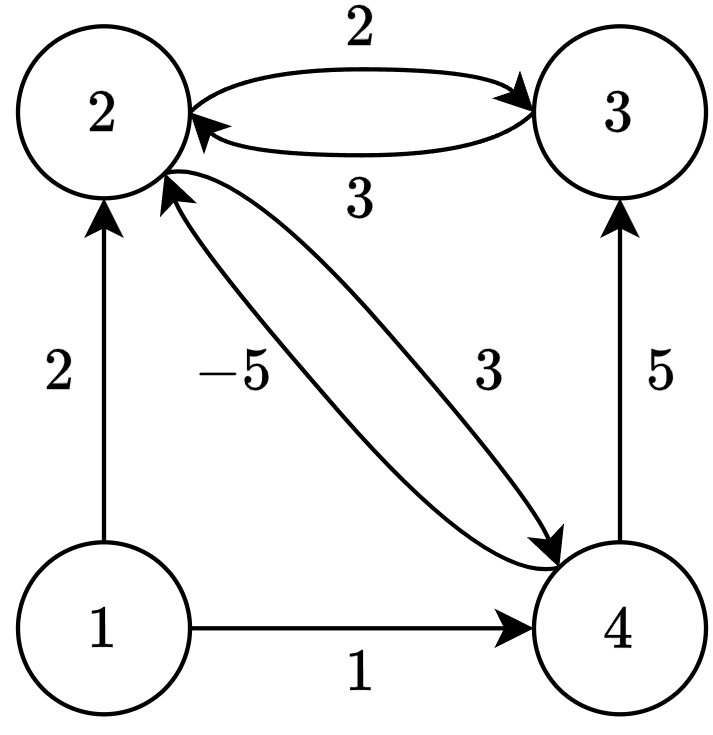
\includegraphics[width=0.2\linewidth]{images/floyd.png}
        \end{figure}
        To initiate the algorithm, we initialize the matrices as follows:
        \[D=\begin{bmatrix}
            0 & 2 & \infty & 1 \\
            \infty & 0 & 3 & 3 \\
            \infty & 2 & 0 & \infty \\
            \infty & -5 & 5 & 0 \\
        \end{bmatrix}
        \:\:\:\:\:\:
        P=\begin{bmatrix}
            1 & 1 & 1 & 1 \\
            2 & 2 & 2 & 2 \\
            3 & 3 & 3 & 3 \\
            4 & 4 & 4 & 4 \\
        \end{bmatrix}
        \]
        In the first iteration with $u=1$ (we focus on the first row and first column), the matrices remain unchanged because the triangular operation is consistently satisfied:
        \begin{itemize}
            \item $0=d_{22} < d_{21} + d_{12} = \infty + 2$ (no changes). 
            \item $3=d_{23} < d_{21} + d_{13} = \infty + \infty$ (no changes). 
            \item $3=d_{24} < d_{21} + d_{14} = \infty + 1$ (no changes). 
            \item $2=d_{32} < d_{31} + d_{12} = \infty + 2$ (no changes). 
            \item $0=d_{33} < d_{31} + d_{13} = \infty + \infty$ (no changes). 
            \item $\infty=d_{34} < d_{31} + d_{14} = \infty + 1$ (no changes). 
            \item $-5=d_{42} < d_{41} + d_{12} = \infty + 2$ (no changes). 
            \item $5=d_{43} < d_{41} + d_{13} = \infty + \infty$ (no changes). 
            \item $0=d_{44} < d_{41} + d_{14} = \infty + 1$ (no changes). 
        \end{itemize}
        In the second iteration with $u=2$ (focusing on the second row and second column), the matrices are modified, and the algorithm terminates due to the discovery of a negative-cost arc:
        \begin{itemize}
            \item $0=d_{11} < d_{12} + d_{21} = 2 +\infty $ (no changes). 
            \item $\infty=d_{13} < d_{12} + d_{23} = 2+3$ ($p_{13} \leftarrow p_{23}$). 
            \item $1=d_{14} < d_{12} + d_{24} = 2+3$ (no changes). 
            \item $\infty=d_{31} < d_{32} + d_{21} = 2 + \infty$ (no changes). 
            \item $0=d_{33} < d_{32} + d_{23} = 2+3$ (no changes). 
            \item $\infty=d_{34} < d_{32} + d_{24} = 2+3$ ($p_{34} \leftarrow p_{24}$). 
            \item $\infty=d_{41} < d_{42} + d_{21} = 5 + \infty$ (no changes). 
            \item $5=d_{43} < d_{42} + d_{23} = -5+3$ ($p_{43} \leftarrow p_{23}$). 
            \item $0=d_{44} < d_{42} + d_{24} = -5+3$ (negative cost circuit found). 
        \end{itemize}
    \end{example}

    The algorithm takes as its inputs a directed graph $G = (N,A)$ and an $n \times n$ cost matrix, $C = [c_{ij}]$.
    \begin{algorithm}[H]
        \caption{Floyd-Warshall's algorithm}
            \begin{algorithmic}[1]
                \For {$i \in N$}
                    \For {$j \in N$}
                        \State $p_{ij} \leftarrow i$
                        \State $d_{ij} \leftarrow \begin{cases}
                            0 \:\:\:\:\:\:\:\:\:\:\: i = j \\
                            c_{ij} \:\:\:\:\:\:\:\:\: i \neq j \land (i,j) \in A \\
                            +\infty \:\:\:\:\:\: \textnormal{otherwise}
                        \end{cases}$
                    \EndFor
                \EndFor
                \For {$u \in N$}
                    \For {$i \in N-\{u\}$}
                        \For {$j \in N-\{u\}$}
                            \If {$d_{iu}+d_{uj} \ d_{ij}$}
                                \State $p_{ij} \leftarrow p_{uj}$
                                \State $d_{ij} \leftarrow d_{iu}+d_{uj}$
                            \EndIf
                        \EndFor
                    \EndFor
                    \For {$i \in N$}
                        \If {$d_{ii} < 0$}
                            \State \Return
                        \EndIf
                    \EndFor
                \EndFor
            \end{algorithmic}
    \end{algorithm}
    Given that the triangular operation is executed for all nodes $u$ and for each pair of nodes $i$ and $j$ in the worst-case scenario, the overall time complexity of the Floyd-Warshall algorithm is $O(n^3)$.
    \begin{proposition}
        Floyd-Warshall's algorithm is exact. 
    \end{proposition}
    \begin{proof}
        Let's assume that the nodes of $G$ are numbered from $1$ to $n$. 
        We can verify that when following the node index order, after the $u$-th cycle, the value of $d_{ij}$ (for any $i$ and $j$) corresponds to the cost of the shortest path from $i$ to $j$ with only intermediate nodes in the set ${1,\dots,u}$. 
    \end{proof}

    \subsection{Topological order algorithm}
    The topological order algorithm deals with a directed acyclic graph $G = (N,A)$, where each arc $(i,j) \in A$ has an associated cost $c_ij \in \mathbb{R}$, 
    Given nodes $s$ and $t$, the goal is to determine the shortest or longest path from $s$ to $t$.
    Directed acyclic graphs possess a crucial property known as topological order, where the nodes in any such graph $G$ can be indexed in a way that for each arc $(i, j) \in A$, we have $i < j$. 
    This topological order property can be leveraged in an efficient dynamic programming algorithm to find shortest or longest paths in directed acyclic graphs.
    To apply the algorithm to a graph $G = (N,A)$, represented using lists of predecessors $\delta^{-}(v)$ and successors $\delta^{+}(v)$ for each node $v$, follow these steps:
    \begin{enumerate}
        \item Assign the smallest positive integer that has not been assigned to a node $v \in N$ with $\delta^{-}(v)=\varnothing$. 
        \item Delete node $v$ with all its incident arcs.
        \item Repeat from step one until there are nodes remaining in the current sub-graph.
    \end{enumerate}
    The complexity of this algorithm is $O(m)$, where $m$ is the cardinality of $A$ (the number of arcs), because each node and arc are considered at most once.
    \begin{example}
        Here's a graphical illustration of the algorithm:
        \begin{figure}[H]
            \centering
            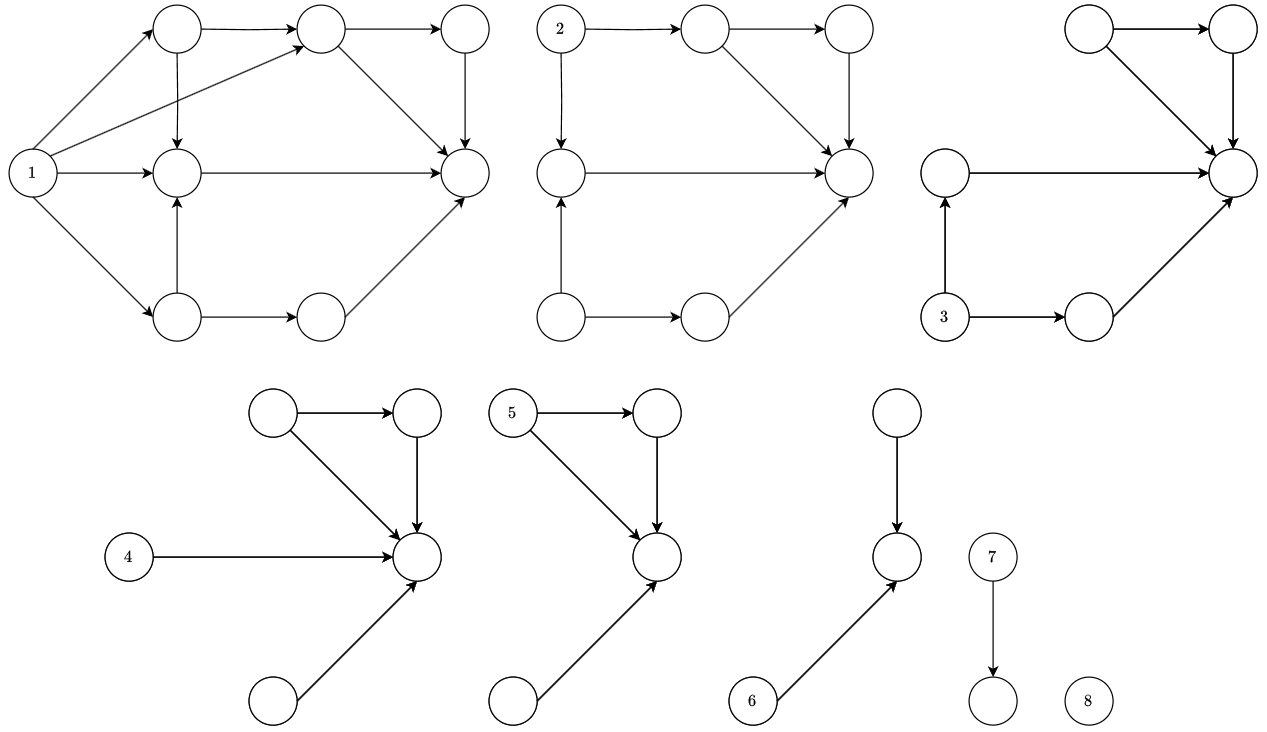
\includegraphics[width=0.8\linewidth]{images/spath.png}
        \end{figure}
    \end{example}

    \subsection{DAGs' dynamic programming algorithm}
    Any shortest path from 1 to $\pi_t$, with at least two arcs, can be subdivided into two parts: $\pi_t$ and $(i,t)$, where $\pi_t$ is the shortest sub-path from $s$ to $i$. 
    For each node  $i=1,\dots,t$, let $L_i$ denote the cost of the shortest path from $1$ to $i$. 
    Therefore, we can express $L_t$as follows:
    \[L_t=\min_{(i,t) \in \delta^{-}(t)}\{L_i+c_{it}\}\]
    This minimum is taken over all possible predecessors $i$ of $t$.
    If the graph $G$ is directed, acyclic, and topologically ordered, the only possible predecessors of $t$ in the shortest path $\pi_t$ from 1 to $t$ are those nodes with an index $i$ less than $t$. 
    Consequently:
    \[L_t=\min_{i<t}\{L_i+c_{it}\}\]
    However, in a graph with cycles, any node other than $t$ can be a predecessor of $t$ in $\pi_t$.  

    For Directed Acyclic Graphs (DAGs) whose nodes are topologically ordered, $L_{t-1},\dots,_L1$ satisfy the same type of recursive relations:
    \[L_{t-1}=\min_{i<t-1}\{L_i+c_{i,t-1}\};\dots;L_2=\min_{i=1}\{L_i+c_i2\}=L_1+c_{12};L_1=0\]
    These relations can be solved in reverse order:
    \[L_1=0;L_2=L_1+c_{12};\dots;L_{t}=\min_{i<t-1}\{L_i+c_{t}\}\]
    \begin{example}
        Consider the following graph:
        \begin{figure}[H]
            \centering
            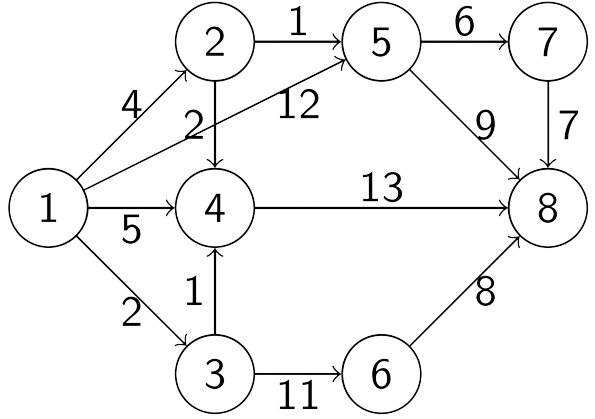
\includegraphics[width=0.4\linewidth]{images/DAG.png}
        \end{figure}
        To find the shortest paths in a Directed Acyclic Graph (DAG) using dynamic programming, follow this workflow:
        \begin{itemize}
            \item $L_1=0 \rightarrow \textnormal{pred}_1=1$
            \item $L_2=L_1+c_{12}=4 \rightarrow \textnormal{pred}_2=1$
            \item $L_3=L_1+c_{13}=2 \rightarrow \textnormal{pred}_3=1$
            \item $L_4=\min_{i=1,2,3}\{L_i+c_{i4}\}=\min{5,6,3}=3 \rightarrow \textnormal{pred}_4=3$
            \item $L_5=\min_{i=1,2}\{L_i+c_{i5}\}=\min{12,5}=5 \rightarrow \textnormal{pred}_5=2$
            \item $L_6=L_3+c_{36}=13 \rightarrow \textnormal{pred}_6=3$
            \item $L_7=L_5+c_{57}=11 \rightarrow \textnormal{pred}_7=5$
            \item $L_8=\min_{i=4,5,6,7}\{L_i+c_{i8}\}=\min{16,14,21,18}=14 \rightarrow \textnormal{pred}_8=5$
        \end{itemize}
    \end{example}
    \begin{algorithm}[H]
        \caption{Dynamic programming to find the shortest paths in DAGs}
            \begin{algorithmic}[1]
                \State Sort the nodes of $G$ topologically
                \State $L_1 \leftarrow 0$
                \For {$j=2,\dots,n$}
                    \State $L_j \leftarrow \min\{L_i+c_{ij}|(i,j) \in \delta^{-}(j) \land i < j\}$
                    \State $pred_j \leftarrow v \: \textnormal{such that} \: (v,j)=\textnormal{argmin} \{L_i+c_{ij}|(i,j) \in \delta^{-}(j) \land i < j\}$
                \EndFor
            \end{algorithmic}
    \end{algorithm}
    As the nodes are topologically ordered, each node and each arc is processed exactly once, resulting in a time complexity of $O(m)$, where $m$ represents the cardinality of $A$ (the number of arcs).    
    
    The same algorithm can also be applied to find the longest path using the following formula:
    \[L_t=\max_{i<t}\{L_i+c_{it}\},\dots\]

    \begin{proposition}
        The dynamic programming algorithm for DAGs is exact. 
    \end{proposition}
    \begin{proof}
        This phenomenon can be attributed to the optimality principle.
        For any shortest (longest) path from node from 1 to $t,\pi_t$, there exists a pair of nodes $i$ and $j$, where $i < j$,  such that the path can be partitioned into two parts: $\pi_i$ and $(i,t)$, where $\pi_i$ represents the minimum (maximum) length from $s$ to $i$.
    \end{proof}

    \subsection{Project planning algorithm}
    \begin{definition}
        A \emph{project}  comprises a collection of $m$ activities with an associated duration. 
        Specifically, activity $A_i$ has an estimated duration of $d_j \geq 0, i=1,\dots,m$. 

        Certain pairs of activities are governed by \emph{precedence constraint}. 
        A notation such as $A_i \varpropto A_j$ signifies that the commencement of $A_j$ is contingent upon the completion of $A_i$. 
    \end{definition}
    A project can be conveniently represented using a directed graph $G = (N, A)$, where each arc corresponds to an activity, and the length of the arc signifies the duration of the associated activity.
    In order to account for the precedence constraints, the arcs must be arranged in a manner such that the notation $A_i \varpropto A_j$ implies the existence of a directed path where the arc associated with $A_i$ precedes the arc associated with $A_j$.
    This ensures the proper sequencing of activities.
    In this context, a node $v$ marks an event corresponding to the end of all the activities $(i,v) \in \delta^{-}(v)$, consequently, it indicates the potential beginning of all activities $(v,j) \in \delta^{+}(v)$. 
    To enhance the representation of graph $G$ we use additional nodes that adheres to the following criteria:
    \begin{itemize}
        \item It includes a distinct initial node $s$, symbolizing the project's start event.
        \item It incorporates a unique final node $t$, representing the project's completion event.
        \item It maintains a structure where multiple arcs with the same endpoints are avoided, ensuring clarity and consistency in the representation. 
    \end{itemize}
    \begin{property}
        The directed graph G representing any project is acyclic (it is a DAG). 
    \end{property}
    \begin{proof}
        By contradiction, if $A_{i1}\varpropto A_{12},\dots,A_{jk}\varpropto A_{ki}$ there would be a logical inconsistency. 
    \end{proof}  
    \begin{example}
        A project can be described as follows:
        \begin{figure}[H]
            \centering
            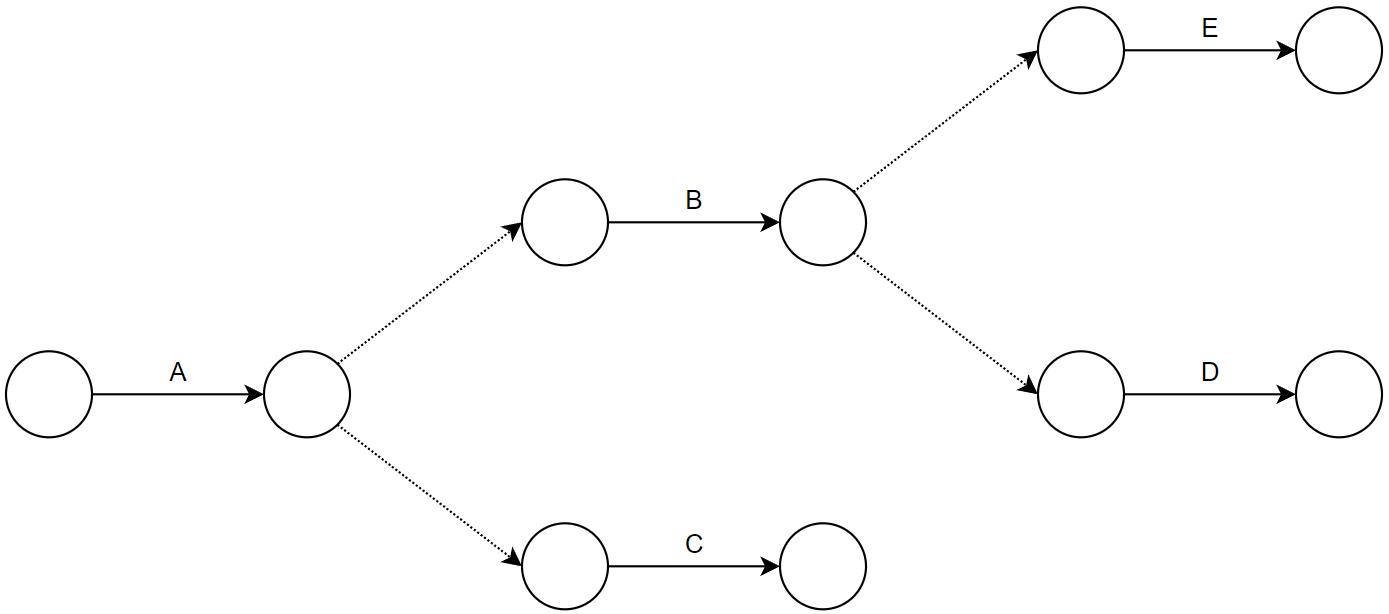
\includegraphics[width=0.5\linewidth]{images/project.png}
        \end{figure}
        While it is possible to simplify this graph by contracting some arcs, care must be taken to avoid introducing unwanted precedence constraints. 
        The correctly contracted graph appears as follows:
        \begin{figure}[H]
            \centering
            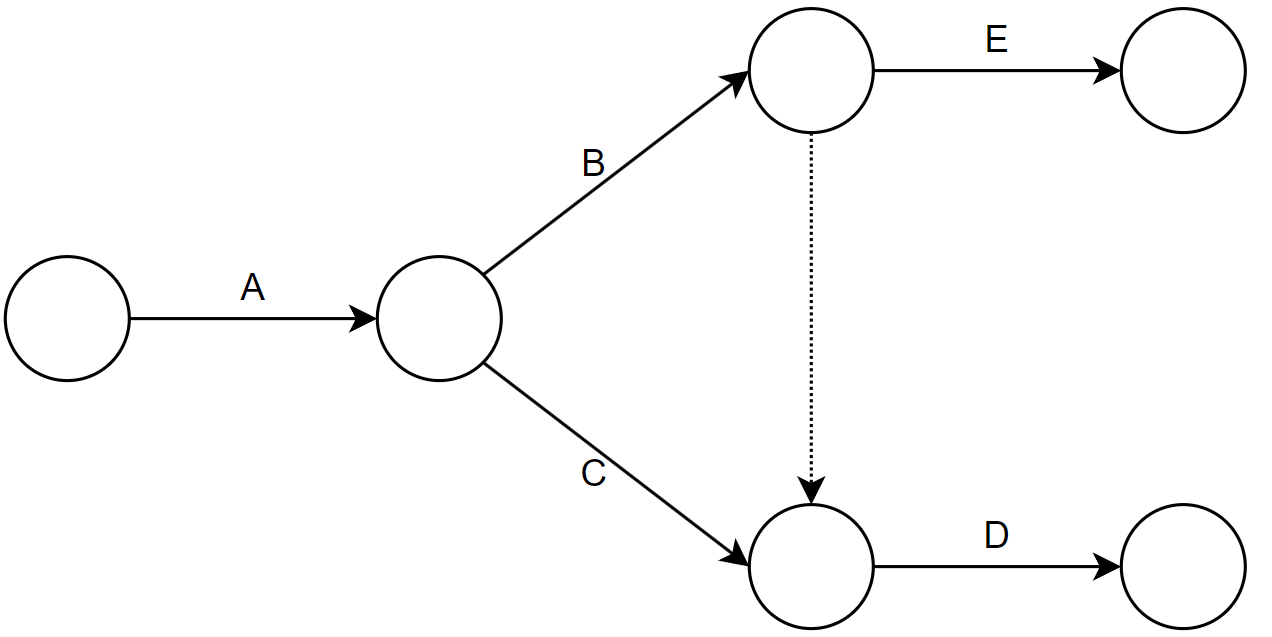
\includegraphics[width=0.4\linewidth]{images/cproject.png}
        \end{figure}
        Additionally, we can introduce the initial and final nodes to create a more structured representation:
        \begin{figure}[H]
            \centering
            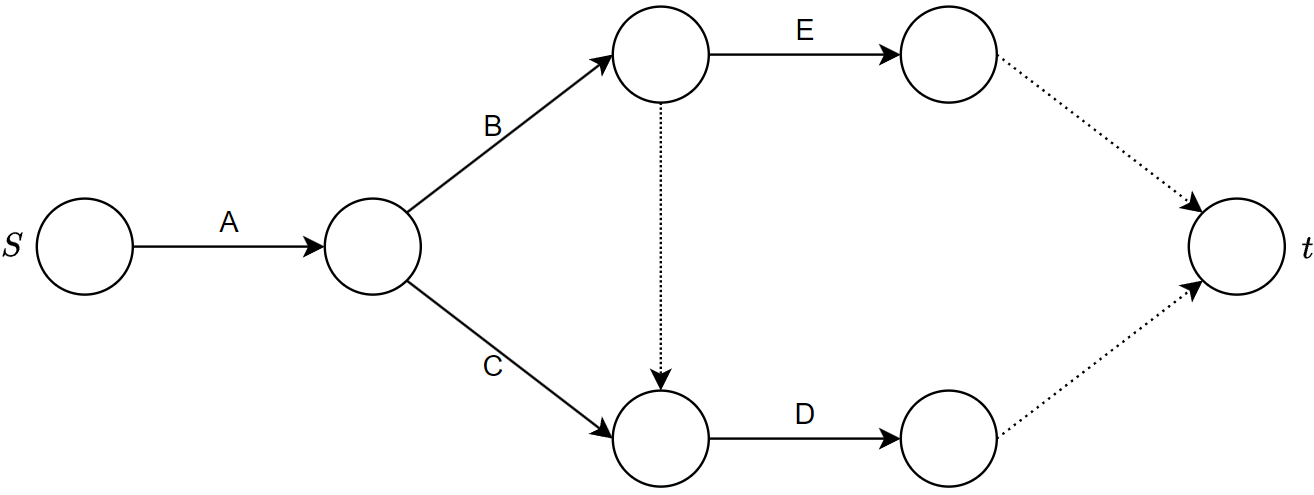
\includegraphics[width=0.5\linewidth]{images/fproject.png}
        \end{figure}
    \end{example}
    The problem to be addressed is as follows: given a project, the task is to schedule the activities in a manner that minimizes the total duration of the project.
    \begin{property}
        The minimum overall project duration is the length of the longest path from $s$ to $t$. 
    \end{property}
    \begin{proof}
        Since any $s-t$ path represents a sequence of activities that must be executed in the specified order, its length provides a lower bound on the minimum overall project duration. 
    \end{proof}  
    To address this problem, we can employ the Critical Path Method (CPM), which accomplishes the following:
    \begin{itemize}
        \item Establishes a schedule to minimize the overall project duration.
        \item Determines the slack for each activity.
    \end{itemize}
    The algorithm takes as input the project's representation graph $G$ and seeks to identify a topological order of the nodes. 
    The steps involved are as follows:
    \begin{enumerate}
        \item Traverse the nodes in ascending order of indices.
            For each node $h \in N$, calculate the earliest time, denoted as $T_{min_h}$, at which the event associated with node $h$ can occur ($T_{min_n}$ corresponds to the minimum project duration).
        \item Traverse the nodes in descending order of indices.
            For each node $h \in N$, compute the latest time, denoted as $T_{max_h}$, at which the event associated with node h can occur without causing a delay in the project's completion beyond $T_{min_n}$.
        \item For each activity $(i,j) \in A$, determine the slack, denoted as $\sigma_{ij}$, using the formula: 
            \[\sigma_{ij}=T_{max_j}-T_{max_i}-d_{ij}\]
    \end{enumerate}
    \begin{example}
        Consider the following project:
        \begin{table}[H]
            \centering
            \begin{tabular}{ccc}
            \hline
            \textbf{Activity} & \textbf{Duration} & \textbf{Predecessors} \\ \hline
            A                 & 3                 & -                     \\
            B                 & 2                 & A                     \\
            C                 & 3                 & A                     \\
            D                 & 3                 & C                     \\
            E                 & 4                 & B, C                  \\
            F                 & 3                 & B                     \\
            G                 & 1                 & E, D                  \\
            H                 & 4                 & C                     \\
            I                 & 2                 & F                     \\ \hline
            \end{tabular}
        \end{table}
        With the following precedence constraints:
        \[A \varpropto B,A \varpropto C,C \varpropto D,B \varpropto E, C \varpropto E,B \varpropto F,E \varpropto G,D \varpropto G,C \varpropto H,F \varpropto I\]
        The objective is to determine the minimum overall duration of the project and calculate the slack for each activity. 
        To do this, we start by creating a graph associated with the given problem:
        \begin{figure}[H]
            \centering
            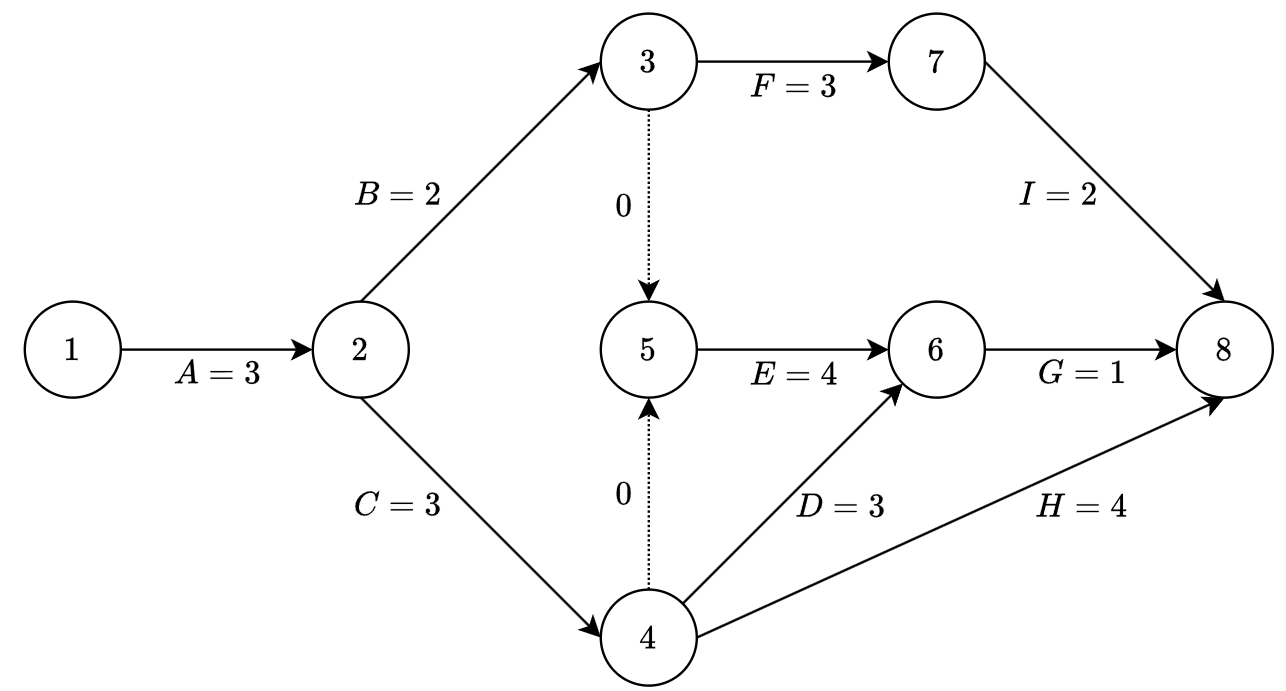
\includegraphics[width=0.5\linewidth]{images/eproject.png}
        \end{figure}
        The first two phases of the CPM algorithm result in the following graphs:
        \begin{figure}[H]
            \centering
            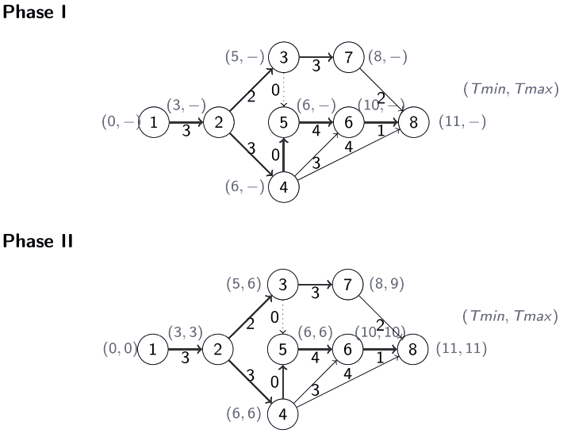
\includegraphics[width=0.75\linewidth]{images/aproject.png}
        \end{figure}
        \begin{figure}[H]
            \centering
            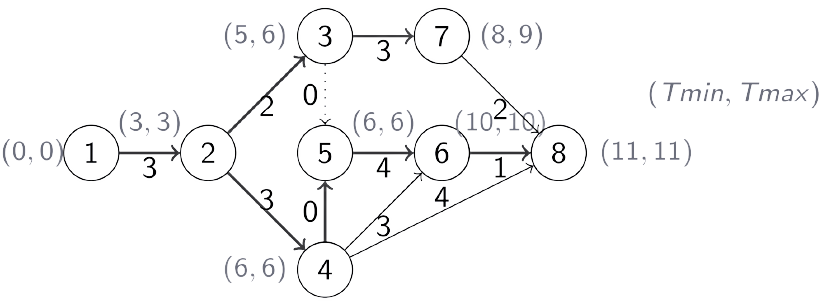
\includegraphics[width=0.75\linewidth]{images/aproject1.png}
        \end{figure}
        As a result, the longest path that is critical, and hence determines the minimum project duration, is $(1,2,4,5,6,8)$.
    \end{example}
    The algorithm takes as inputs a graph $G = (N,A)$, where $n= \left\lvert N \right\rvert $, and the duration $d_{ij}$ assigned to each $(i,j) \in A$. 
    \begin{algorithm}[H]
        \caption{Algorithm for the critical path method}
            \begin{algorithmic}[1]
                \State Sort the nodes of $G$ topologically
                \State $T_{min_1} \leftarrow 0$
                \For {$j=2,\dots,n$}
                    \State $T_{min_j} \leftarrow \max\{T_{min_i}+d_{ij}|(i,j) \in \delta^{-}(j)\}$
                \EndFor
                \State $T_{max_n} \leftarrow T_{min_n}$
                \For {$i=n-1,\dots,1$}
                \State $T_{max_j} \leftarrow \min\{T_{max_j}-d_{ij}|(i,j) \in \delta^{+}(j)\}$
                \EndFor
            \end{algorithmic}
    \end{algorithm}
    The algorithm's time complexity is $O(m)$, where $m =\left\lvert A\right\rvert$. 
    \begin{definition}
        An activity $(i,j)$ with zero slack, which means that:
        \[\sigma_{ij}=T_{max_j}-T_{min_i}-d_{ij}=0\]
        is considered \emph{critical}. 

        A \emph{critical path} is defined an $s-t$ path only composed of critical activities (it always exists).
    \end{definition}

    To determine the slack of a project, another approach is to use Gantt charts, which were initially introduced by Henry Gantt in 1910. 
    These charts offer a visual representation of the project's timeline.
    \begin{example}
        The outcome of the previous example is as follows:
        \begin{table}[H]
            \centering
            \begin{tabular}{cccc}
            \hline
            $(i,j)$ & $d_{ij}$ & $T_{min_i}$ & $T_{max_j}$ \\ \hline
            A       & 3        & 0           & 3           \\
            B       & 2        & 3           & 6           \\
            C       & 3        & 3           & 6           \\
            D       & 3        & 6           & 10          \\
            E       & 4        & 6           & 10          \\
            F       & 3        & 5           & 9           \\
            G       & 1        & 10          & 11          \\
            H       & 4        & 6           & 11          \\
            I       & 2        & 8           & 11          \\ \hline
            \end{tabular}
        \end{table}
        These results can be illustrated using a Gantt chart as shown below:
        \begin{figure}[H]
            \centering
            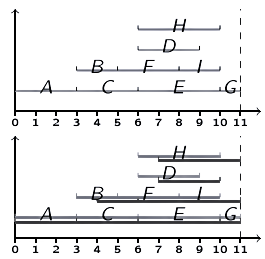
\includegraphics[width=0.25\linewidth]{images/Gantt.png}
        \end{figure}
    \end{example}

    \section{Minimum network flow problem}
    The network flow problem involves efficiently distributing a particular product from a set of sources to a set of users in order to optimize a predefined objective function.
        \begin{definition}
        A network is a directed and connected graph $G = (V,A)$ with a source $s \in V$ and a sink $t \in V$, with $s \neq t$, and a capacity $k_{ij} \geq 0$ for each arc 
        $(i,j) \in A$. 

        A \emph{feasible flow} $x$ from $s$ to $t$ is a vector $x \in \mathbb{R}^m$ with a component $x_{ij}$ for each arc $(i,j) \in A$ satisfying the capacity constraints:
        \[0 \leq x_{ij} \leq k_{ij} \:\:\:\:\:\: \forall (i,j) \in A\]
        and the flow balance constraints at each intermediate node $u \in V (u \neq s,t)$: 
        \[\sum_{(i,u)\in \delta^{-}(u)}x_{iu}=\sum_{(u,j)\in \delta^{+}(u)}x_{uj} \:\:\:\:\:\: \forall u \in N-\{s,t\}\]

        The \emph{value of flow} $x$ is:
        \[\varphi = \sum_{(s,j) \in \delta^{+}(s)} x_{sj}\]

        Given a network and a feasible flow $x$, an arc $(i,j) \in A$ is \emph{saturated} if $x_{ij} = k_{ij}$. 

        Given a network and a feasible flow $x$, an arc $(i,j) \in A$ is \emph{empty} if $x_{ij} = 0$. 
    \end{definition}
    In the network flow problem, we are given a network $G = (V,A)$ with integer capacities $k_{ij}$ for each arc $(i,j) \in A$, and two designated nodes $s,t \in V$. 
    The goal is to determine a feasible flow from $s$ to $t$ with the maximum value.

    In cases where there are multiple sources and sinks with a single type of product, dummy nodes $s^{*}$ and $t^{*}$ can be introduced. 
    The linear programming model for this problem aims to maximize $\max \varphi$, subject to the following constraints:
    \[\sum_{(u,j)\in \delta^{+}(u)}x_{uj}-\sum_{(i,u)\in \delta^{-}(u)}x_{iu}=
    \begin{cases}
        \varphi \:\:\:\:\:\:\:\:\: u=s    \\
        -\varphi \:\:\:\:\:\: u=t   \\
        0 \:\:\:\:\:\:\:\:\:\: \textnormal{otherwise}
    \end{cases}\]
    Here, $\varphi$ represents the value of the feasible flow $x$, $0 \leq x_{ij} \leq k_{ij}$ with $\varphi,x_{ij} \in \mathbb{R}$, and $(i,j) \in A$.
    \begin{definition}
        A \emph{cut separating $s$ from $t$} is $\delta(S)$ of $G$ with $s \in S \subset V$ and $t \in V-S$. There are $2^{n-2}$ cuts separating $s$ from $t$, where 
        $n=\left\lvert V \right\rvert $.

        The \emph{capacity of the cut} $\delta(S)$ induced by $S$ is equal to: 
        \[k(S)=\sum_{(i,j)\in \delta^{+}(S)}k_{ij}\]

        Given a feasible flow $x$ from $s$ to $t$ and a cut $\delta(S)$ separating $s$ from $t$, the \emph{value of the feasible flow x through the cut $\delta(S)$} is: 
        \[\varphi(S)=\sum_{(i,j)\in \delta^{+}(S)}x_{ij} - \sum_{(i,j)\in \delta^{-}(S)}x_{ij}\]
    \end{definition}
    With this notation, the value of the flow $x$ is represented as $\varphi = \varphi(\{s\})$. 
    \begin{property}
        Given a feasible flow $x$ from $s$ to $t$, for each cut $\delta(S)$ separating $s$ from $t$, we have $\varphi(S)=\varphi(\{s\})$.
    \end{property}
    \begin{property}
        For every feasible flow $x$ from $s$ to $t$ and every cut $\delta(S)$, with $S \subseteq V$, separating $s$ from $t$, we have $\varphi(S) \leq k(S)$:
        \[\varphi(S) \leq k(S)\]
        This expression signifies that the flow's value is either less than or equal to the capacity of the cut.
    \end{property}
    \begin{proof}
        According to the definition of the flow value through the cut $\delta(S)$, we express it as:
        \[\varphi(S)=\sum_{(i,j) \in \delta^{+}(S)}x_{ij}-\sum_{(i,j) \in \delta^{-}(S)}x_{ij}\]
        Furthermore, considering that $0 \leq x_{ij } \leq k_{ij}$ for any edge $(i, j) \in A$, we can establish:
        \[\sum_{(i,j) \in \delta^{+}(S)}x_{ij}-\sum_{(i,j) \in \delta^{-}(S)}x_{ij} \leq \sum_{(i,j) \in \delta^{+}(S)}k_{ij}=k(S)\]
        Hence, it follows that $\varphi(S) \leq k(S)$.
    \end{proof}
    \begin{example}
        The value of the feasible flow $x$ passing through the cut $\delta(S)$  in the graph is illustrated below:
        \begin{figure}[H]
            \centering
            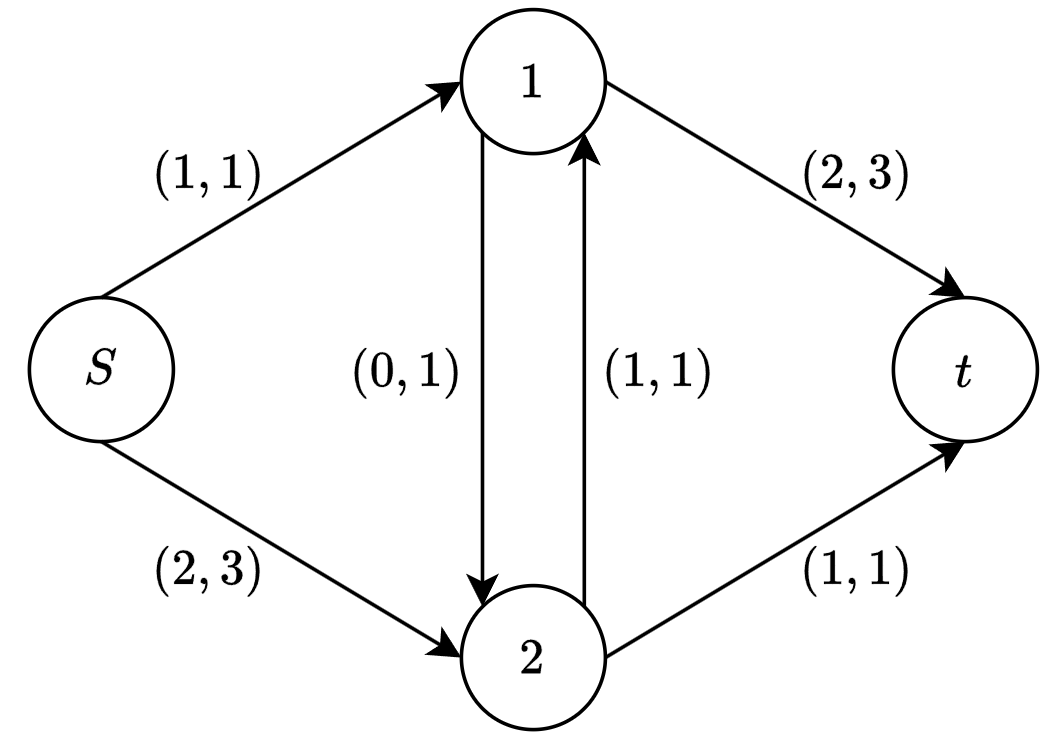
\includegraphics[width=0.25\linewidth]{images/flow.png}
        \end{figure}
        \[\varphi(\{s,1\})=2+0+2-1=3\]
        The remaining values are as follows: 
        \[\delta(\{s,1\})=\{(s, 2),(1,2),(1, t)\}\]
        \[k(S)=7\]
    \end{example}
    If $\varphi(S) = k(S)$ for a subset $S \subseteq V$ containing the source $s \in S$ and excluding the destination $t \notin S$, then the flow $x$ attains its maximum value, and the cut $\delta(S)$ represents the minimum capacity. 
    The property $\varphi(S) \leq k(S)$ for any feasible flow $x$ and any cut $\delta(S)$ that separates $s$ from $t$ signifies a weak duality connection between two problems:
    \begin{itemize}
        \item Determining a feasible flow of maximum value in a graph $G = (V, A)$ with integer capacities on the arcs and source-destination pair $s, t \in V$.
        \item Identifying a cut (one that separates $s$ from $t$) of minimum capacity in a graph $G = (V, A)$ with integer arc capacities and source-destination pair $s, t \in V$.
    \end{itemize} 
    The idea of the Ford-Fulkerson's algorithm to find network flows is as follows: start from a feasible flow $x$ and try to iteratively increase its value $\varphi$ by sending, at each iteration, an additional amount of product along an undirected path from $s$ to $t$ with a strictly positive residual capacity. 
    If the arc $(i,j)$ is not saturated, we can increase $x_{ij}$. 
    If $(i,j)$ is not empty, we can decrease $x_{ij}$ while respecting $0 \leq x_{ij} \leq k_{ij}$. 
    \begin{definition}
        A path $P$ from $s$ to $t$ is an \emph{augmenting path} with respect to the current feasible flow $x$ if $x_{ij} <  k_{ij}$ for any
        forward arc $x_{ij}>0$ for any backward arc. 
    \end{definition}
    Given a feasible flow $x$ for $G=(V,A)$, we create the residual network denoted as $\overline{G}=(V,\overline{A})$ associated to $x$. 
    This residual network encompasses all conceivable adjustments to the flow $x$: 
    \begin{itemize}
        \item If $(i,j) \in A$ is not empty $(i,j) \in \overline{A}$ with $\overline{k}_{ij}=x_{ij}>0$.
        \item If $(i,j) \in A$ is not saturated $(i,j) \in \overline{A}$ with $\overline{k}_{ij}=k_{ij}-x_{ij}>0$
    \end{itemize}
    Here, $\overline{k}_{ij}$ is termed residual capacity. 
    \begin{example}
        To determine the residual capacity of the graph depicted below, we follow this procedure:
        \begin{figure}[H]
            \centering
            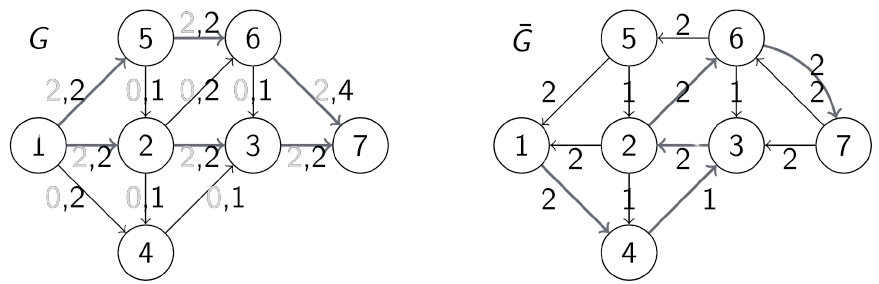
\includegraphics[width=0.75\linewidth]{images/residual1.png}
        \end{figure}
        Afterward, we update the flow and once more compute the residual capacity:
        \begin{figure}[H]
            \centering
            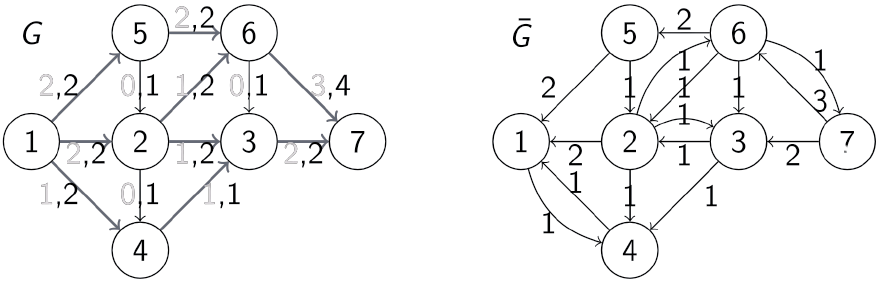
\includegraphics[width=0.75\linewidth]{images/residual2.png}
        \end{figure}
        This process is repeated:
        \begin{figure}[H]
            \centering
            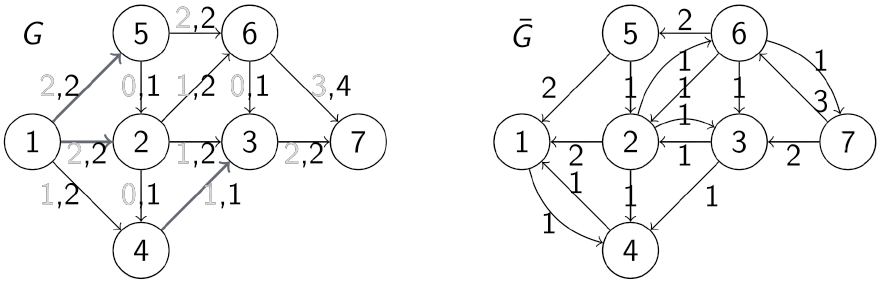
\includegraphics[width=0.75\linewidth]{images/residual3.png}
        \end{figure}
        However, since we are unable to identify additional paths, we conclude that the flow is now $\phi=5$.
    \end{example}
    \begin{proposition}
        Ford-Fulkerson's algorithm is exact. 
    \end{proposition}
    \begin{proof}
        A feasible flow denoted as $x$  achieves its maximum value if and only if the destination node $t$ cannot be reached from the source node $s$ in the residual network associated with flow $x$. 
        If an augmenting path exists, then flow $x$ is not optimal for achieving the maximum value.
        When $t$ is not reachable from $s$, it implies the presence of a cut in the residual network $\overline{G}$ such that $\delta^{+}_{\overline{G}}(S^{*})=\varnothing$. 
        By the definition of $\overline{G}$  every edge $(i,j) \in \delta^{+}_{G}(S^{*})$ is saturated, and every edge in $\delta^{-}_{G}(S^{*})$ is empty. 
        Consequently,
        \[\phi(S^{*})=\sum_{(i,j) \in \delta^{+}_{G}(S^{*})}{x_{ij}}-\sum_{(i,j) \in \delta^{-}_{G}(S^{*})}{x_{ij}}= \sum_{(i,j) \in \delta^{+}_{G}(S^{*})}{k_{ij}}=k(S^{*})\]
        According to weak duality, it follows that $\phi(S) < k(S)$ for all feasible flows $x$ and $\forall S \subset V$ with $s \in S$, $t \notin S$. 
        Therefore, the flow $x$ has maximum value and the cut induced by $S^{*}$ represents the minimum capacity.
    \end{proof}
    \begin{theorem}
        The value of a feasible flow of maximum value is equal to the capacity of a cut of minimum capacity.
    \end{theorem}
    The algorithm takes as its inputs a graph denoted as $G=(V,A)$ with non-zero capacities $k_{ij}>0$ for all edges $(i,j) \in A$, where $t \in N$. 
    \begin{algorithm}[H]
        \caption{Ford-Fulkerson's algorithm}
            \begin{algorithmic}[1]
                \State $x \leftarrow 0$
                \State $\phi \leftarrow 0$
                \State $\textnormal{optimum} \leftarrow \textnormal{false}$
                \While {optimum = true}
                    \State Build residual network $\overline{G}$ associated to $x$
                    \State $P \leftarrow$ path from $s$ to $t$ in $\overline{G}$
                    \If {$P$ is not defined}
                        \State optimum $\leftarrow$ true
                    \Else
                        \State $\delta \leftarrow \min\{\overline{k}_{ij}|(i,j) \in P\}$
                        \State $\phi \leftarrow \phi + \delta$
                        \For {$(i,j) \in P$}
                            \If {$(i,j)$ is a forward arc}
                                \State $x_{ij} \leftarrow x_{ij}+\delta$
                            \Else 
                                \State $x_{ij} \leftarrow x_{ij}-\delta$
                            \EndIf
                        \EndFor
                    \EndIf
                \EndWhile
            \end{algorithmic}
    \end{algorithm}
    The algorithm's total complexity is $O(m^2k_{max})$. 
    The space complexity of the algorithm is $O(m\log{k_{max}})$. 
    To render the algorithm polynomial, one can seek an augmenting path with the minimal number of arcs.

    \subsection{Minimum cost flow problem}
    In the context of a network with unit costs denoted as $c_{ij}$ or each arc  $(i,j)$ and a specified value $\phi > 0$the objective is to find a feasible flow from source $s$ to destination $t$ with a value of $\phi$ while minimizing the total cost.
    To address this problem, the approach involves initiating from a feasible flow $x$ with a value of $\phi$ and dispatching an additional quantity of goods within the residual network through cycles characterized by negative costs.
    
    \subsection{Assignment problem}
    \begin{definition}
        Given an undirected bipartite graph $G=(V,E)$, a \emph{matching} $M \subseteq E$ is a subset of non-adjacent edges. 
    \end{definition}
    \begin{figure}[H]
        \centering
        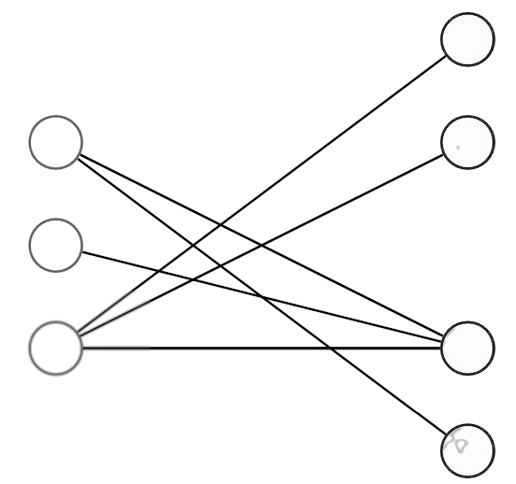
\includegraphics[width=0.2\linewidth]{images/matching.png}
    \end{figure}
    Given a bipartite graph $G=(V,E)$, determine a matching with a maximum number of edges. 
    This problem can be reduced to the problem of finding a feasible flow of maximum value from $s$ to $t$ in the following network. 
    There is a correspondence between the feasible flow of value $\varphi$ and the matching containing $\varphi$ edges. 

    \section{Traveling salesman problem}
    Given a directed graph $G=(N,A)$ with cost $c_{ij} \in \mathbb{Z}$ for each are $(i,j) \in A$, determine a circuit of minimum total cost visiting every node exactly once. 
    \begin{definition}
        A \emph{Hamiltonian circuit} $C$ of $G$ is a circuit that visits every node exactly once. 
    \end{definition}
    Therefore, by representing $H$ as the set encompassing all Hamiltonian circuits within graph $G$, the problem can be formulated as:
    \[\min_{C \in H}{\sum_{(i,j) \in C}{c_{ij}}}\]
    It's important to note that this problem is classified as $\mathcal{N}\mathcal{P}$-hard. 

\newpage 

\chapter{Linear programming}
    \section{Introduction}
    \begin{definition}
        A \emph{linear programming problem} is an optimization problem defined as follows:
        \begin{align*}
            \min                      \:&\:f(x)           \\
            \textnormal{such that }     &\: x \in x \subseteq \mathbb{R}^n \rightarrow \mathbb{R} 
        \end{align*}
        Where: 
        \begin{itemize}
            \item The objective function, denoted as $f:x \rightarrow \mathbb{R}$, is linear. 
            \item The feasible region $x$ is described as:
                \[x=\{x\in\mathbb{R}^n|g_i(x)r_i0\land i\in(1,m)\}\]
                Where $r_i$ takes values from $\{=,\geq,\leq\}$, and $g_i:\mathbb{R}^n\rightarrow\mathbb{R}$ represents linear functions for $i=1,\dots,m$.
        \end{itemize}
    
        An \emph{optimal solution}, denoted as $x^{*} \in \mathbb{R}^n$, of the linear program is defined as satisfying $f(x^{*}) \leq f(x)$ for all $x\in x$
    \end{definition}
    The general form of a linear programming problem can be expressed as follows:
    \[\min{z}=c^Tx\]
    Such that $Ax \geq b$ and $x \geq 0$. 
    In this notation, $x$ represents the vector of decision variables.
    It's important to note that the inequality for the matrix $A$ can be transformed into an equality, and the constraints on the variable values can be relaxed in some instances.
    It's often helpful to convert all linear programming problems into the general form.
    This transformation can be achieved using the following rules:
    \begin{itemize}
        \item To convert a maximization problem into a minimization problem, you can use: 
            \[\max{(c^Tx)}=\min{(-c^Tx)}\]
        \item For $a^Tx \leq b$, you can introduce a slack variable $s$ as: 
            \[a^Tx \leq b \implies
            \begin{cases}
                a^Tx+s=b \\
                s \geq 0
            \end{cases}
            \]
        \item For $a^Tx \geq b$, you can introduce a surplus variable $s$ as: 
            \[a^Tx \geq b \implies 
            \begin{cases}
                a^Tx-s=b \\
                s \geq 0
            \end{cases}
            \]
        \item If a variable $x_{ij}$ is unrestricted in sign, you can represent it as:
            \[\begin{cases}
                x_j=x_j^{+}-x_j^{-} \\
                x_j=x_j^{+},x_j^{-} \geq 0
            \end{cases}
            \]
            After substituting $x_j$ with $x_j^{+}-x_j^{-}$, you can remove $x_j$ from the problem. 
        \item To change the direction of an inequality, you can use the following equivalences:
            \[a^Tx \leq b \textnormal{ is equivalent to } -a^Tx \geq -b\]
            \[a^Tx \geq b \textnormal{ is equivalent to } -a^Tx \leq -b\]
        \item For an equality constraint $a^Tx = b$, you can represent it as:
            \[
            \begin{cases}
                a^Tx \geq b \\
                a^Tx \leq b
            \end{cases}
            \]
    \end{itemize}
    \begin{example}
        Given the following linear programming model, we'll rewrite it in the normal form:
        \begin{align*}
            \max{f(x_1,x_2)}           =&\: 2x_1-3x_2          \\
            \textnormal{such that }     &\: 4x_1-7x_2 \leq 5  \\
                                        &\: 6x_1-2x_2 \geq 4  \\
                                        &\: x_1 \geq 0, x_2 \in \mathbb{R}
        \end{align*}
        We can add two new variables, $x_2=x_3-x_4$, with $x_3,x_4 \geq 0$, and we obtain:
        \begin{align*}
            \max{f(x_1,x_2)}           =&\: 2x_1-3x_2          \\
            \textnormal{such that }     &\: 4x_1-7x_3+7x_4 \leq 5  \\
                                        &\: 6x_1-2x_3+2x_4 \geq 4  \\
                                        &\: x_1,x_2,x_4 \geq 0
        \end{align*}
        Next, we introduce slack and surplus variables $x_5$ and $x_6$, resulting in:
        \begin{align*}
            \max{f(x_1,x_2)}           =&\: 2x_1-3x_2          \\
            \textnormal{such that }     &\: 4x_1-7x_3+7x_4+x_5 = 5  \\
                                        &\: 6x_1-2x_3+2x_4-x_6 = 4  \\
                                        &\: x_1,x_2,x_4,x_5,x_6 \geq 0
        \end{align*}
        Finally, we need to change the sign of the objective function:
        \begin{align*}
            \min{f(x_1,x_2)}           =&\: -2x_1+3x_2          \\
            \textnormal{such that }     &\: 4x_1-7x_3+7x_4+x_5 = 5  \\
                                        &\: 6x_1-2x_3+2x_4-x_6 = 4  \\
                                        &\: x_1,x_2,x_4,x_5,x_6 \geq 0
        \end{align*}
    \end{example}
    The assumptions underlying linear programming models can be summarized as follows:
    \begin{enumerate}
        \item Linearity of the objective function and constraints. 
        \item Proportionality of the objective function and constraints: the contribution of each variable is scaled by a constant. 
        \item Additivity of the objective function and constraints: the overall contribution of all variables is the sum of their individual contributions.
        \item Divisibility: variables are allowed to take rational values, and fractional values are acceptable.
        \item Parameters are considered as constant which can be estimated with a sufficient degree of accuracy. 
    \end{enumerate}
    The linear programming sensitivity analysis is a technique used to assess how an optimal solution reacts to small alterations in parameter values.

    \section{Geometry of linear programming}
    \begin{definition}
        A \emph{level curve} for a value $z$ of a function $f$ is the collection of points in $\mathbb{R}^n$  where the function $f$ remains constant and equals $z$.
    
        A \emph{hyperplane} is described as $H=\{x \in \mathbb{R}^n|a^Tx=b\}$. 
    
        An \emph{affine half-space} is represented as $H=\{x \in \mathbb{R}^n|a^Tx \leq b\}$. 
    \end{definition}
    Every inequality constraint defines an affine half-space within the variable space.
    \begin{definition}
        The feasible region $x$  in any linear programming problem forms a \emph{polyhedron}, denoted as $P$. 
    
        A subset $S \subseteq \mathbb{R}^n$ is considered \emph{convex} if, for any pair $y^1,y^2 \in S$, the entire line segment connecting $y^1$ and $y^2$ is contained within $S$. 
    
        The line segment defined by $y^1$ and $y^2 $ in $ S$, encompassing all \emph{convex combinations} of $y^1$ and $y^2$, is denoted as:
        \[[y^1,y^2]=\{x \in \mathbb{R}^n|x=\alpha y^1+(1-\alpha)y^2 \land \alpha \in [0,1]\} \]
    \end{definition}
    \begin{property}
        A polyhedron $P$ is a convex set of $\mathbb{R}^n$. 
    \end{property}
    This occurs because each half-space is inherently convex, and the intersection of a finite number of convex sets likewise forms a convex set.
    
    \begin{definition}
        A \emph{vertex} of $P$ is a point $P$ that cannot be represented as a convex combination of two other distinct points of $P$. 
    \end{definition}
    In terms of algebraic expression, a vertex is defined as:
    \[x= \alpha y^1+(1-\alpha)y^2, \alpha \in [0,1], y^1,y^2 \in P \implies x=y^1 \lor x=y^2\]
    \begin{property}
        A non-empty polyhedron $P=\{x \in \mathbb{R}^n|Ax=b,x \geq 0\}$ (in standard form) or $P=\{x \in \mathbb{R}^n|Ax=b,x \geq 0\}$ (in canonical form) possesses a finite number ($n \geq 1$) of vertices. 
    \end{property}
    \begin{definition}
        In the context of a problem $P$, a vector $d \in \mathbb{R}^n$ where $d \neq 0$ is considered an \emph{unbounded feasible direction of P} if, for any  point $x_0 \in P$, the ray defined as $\{x \in \mathbb{R}^n|x=x_0+\lambda d,\lambda \geq 0\}$ remains entirely within $P$.
    \end{definition}
    \begin{theorem}
        Each point $x$ within a polyhedron $P$ can be represented as a convex combination of its vertices $x^1,\dots,x^k$ and, if necessary, an unbounded feasible direction $d$ of $P$: 
        \[x=\alpha_1x^1+\dots+\alpha_kx^k+d\]
        Here, the coefficients $\alpha_i \geq 0$ fulfill the condition $\alpha_1+\dots+\alpha_k=1$. 
    \end{theorem}
    \begin{definition}
        A \emph{polytope} is a type of bounded polyhedron, which means it possesses only one unbounded feasible direction, and that direction is $d=0$. 
    \end{definition}
    Each point $x$ within a polytope $P$ can be represented as a convex combination of its vertices.
    \begin{example}
        The point $x=\alpha_1x^1+\alpha_2x^2+\alpha_3x^3$ can also be expressed in the form $\alpha_1+\alpha_2+\alpha_3=1$ $(d=0)$. 
        \begin{figure}[H]
            \centering
            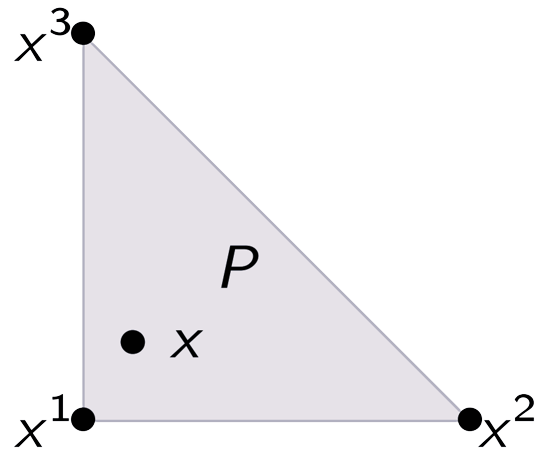
\includegraphics[width=0.2\linewidth]{images/polytope.png}
        \end{figure}
    \end{example}
    The following theorem is recognized as the Fundamental Theorem of Linear Programming.
    \begin{theorem}
        Consider a linear programming problem $\min\{c^Tx|x \in P\}$, where $P \subseteq \mathbb{R}^n$ represents a non-empty polyhedron of feasible solutions (in standard or canonical form), one of the following scenarios must hold true:
        \begin{enumerate}
            \item There exists at least one optimal vertex within $P$.
            \item The value of the objective function is unbounded from below over $P$.
        \end{enumerate}
    \end{theorem}
    \begin{proof}[of case one]
        If $P$ contains an unbounded feasible direction $d$ such that $c^Td < 0$, it signifies that $P$ is unbounded, and the objective function values $z=c^Tx$ decrease indefinitely along the direction $d$. 
    \end{proof}
    \begin{proof}[of case two]
        If $P$ does not possess any unbounded feasible direction $d$ such that $c^Td < 0$, meaning that for all directions $d$, we have$c^Td \geq 0$, then any point within $P$ can be expressed as: 
        \[x=\sum_{i=1}^k{\alpha_ix^i + d}\]
        Here, $x^1,\dots,x^k$ are the vertices of $P$, $\alpha_i > 0$ with $\alpha_1+\dots+\alpha_k=1$, and $d = 0$, or $d$ represents an unbounded feasible direction.
        For any point $x \in P$, either $d = 0$ or $c^Td > 0$, which leads to the following inequality:
        \[c^Tx=c^T\left(\sum_{i=1}^{k}{\alpha_ix^i+d}\right)=\sum_{i=1}^{k}{\alpha_ic^Tx^i+c^Td}\geq\min_{i=1,\dots,n}{c^Tx^i}\]
        This is due to the fact that $\alpha_i > 0$ for any $i$, and $\alpha_1+\dots+\alpha_k=1$. 
    \end{proof}
    From this theorem, we can deduce that an interior point $x \in P$ cannot be an optimal solution. 
    Furthermore, in an optimal vertex, all feasible directions lead to worse objective function values.
    This theorem suggests that even though the variables can take fractional values, linear programming can be approached as a combinatorial problem.
    Consequently, it is essential to investigate the vertices of the polyhedron of feasible solutions.
    However, the number of vertices is finite but can often grow exponentially, making graphical methods practical only when $n \leq 3$. 
    \begin{table}[H]
        \centering
        \begin{tabular}{cc}
        \hline
        \textbf{Type}              & \textbf{Example}                                                                                                   \\ \hline
        Unique optimal solution    & \begin{minipage}{.2\textwidth}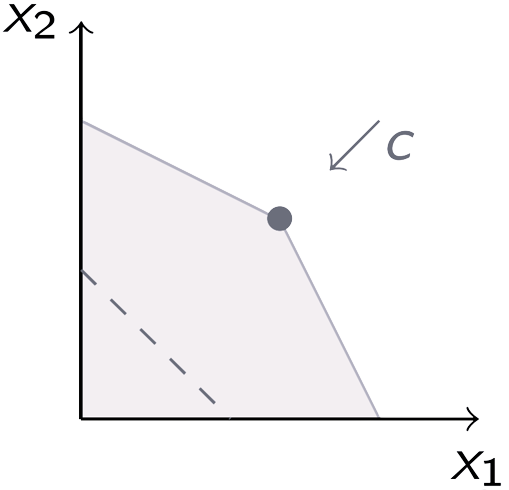
\includegraphics[width=\linewidth, height=30mm]{images/un.png}\end{minipage}         \\ 
        Multiple optimal solutions & \begin{minipage}{.2\textwidth}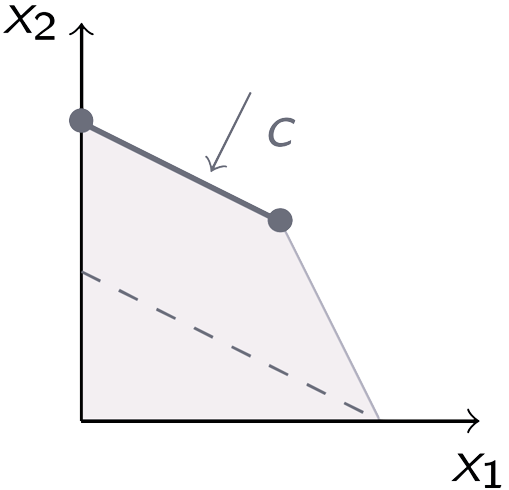
\includegraphics[width=\linewidth, height=30mm]{images/mul.png}\end{minipage}        \\
        Unbounded linear program   & \begin{minipage}{.2\textwidth}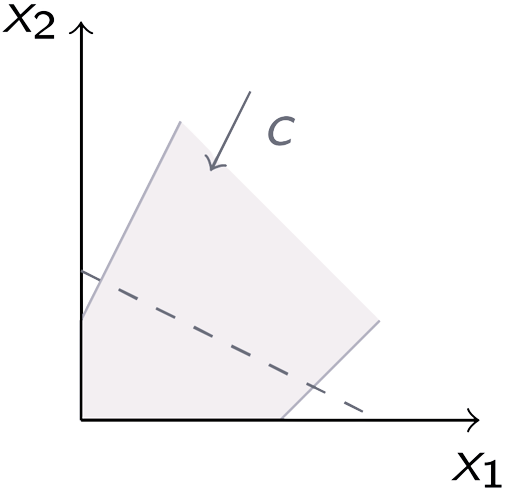
\includegraphics[width=\linewidth, height=30mm]{images/unb.png}\end{minipage}        \\
        Infeasible linear program  & \begin{minipage}{.2\textwidth}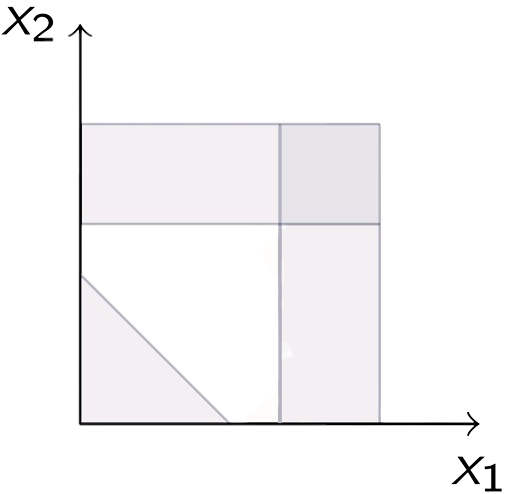
\includegraphics[width=\linewidth, height=30mm]{images/in.png}\end{minipage}         \\     
        \hline       
        \end{tabular}
    \end{table}
    
    \section{Basic feasible solutions}
    Thanks to the Fundamental Theorem of Linear Programming, solving any linear program involves examining the vertices of the polyhedron $P$ containing feasible solutions.
    However, because the geometric definition of a vertex isn't suitable for algorithmic use, we require an algebraic characterization.
    \begin{example}
        Consider the following linear program:
        \begin{align*}
            \min                      \:&\: -x_1-3x_2          \\
            \textnormal{such that }     &\: x_1+x_2 \leq 6  \\
                                        &\: 2x_1+x_2 \leq 8  \\
                                        &\: x_1,x_2 \geq 0
        \end{align*}
        Its graphical representation is shown below:
        \begin{figure}[H]
            \centering
            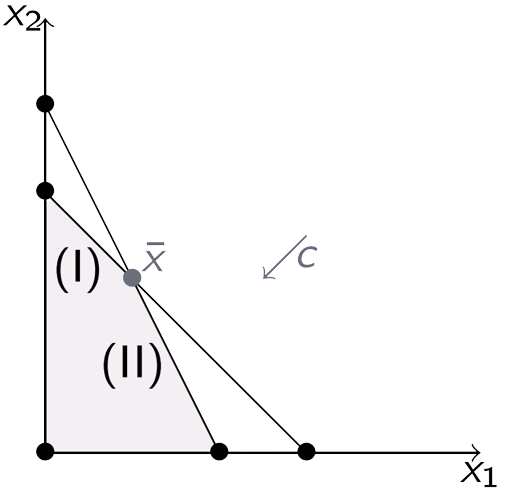
\includegraphics[width=0.25\linewidth]{images/lp.png}
        \end{figure}
        From the graph, it's evident that a vertex corresponds to the intersection of the hyperplanes associated with $n$ inequalities. 
        In this example, the vertex $\overline{x}$ represents the intersection of the first two inequalities, which is the solution to the following system:
        \[
        \begin{cases}
            x_1+x_2=6 \\
            2x_1+x_2=8
        \end{cases}
        \]
        To convert this problem into standard form, we formulate it as:
        \begin{align*}
            \min                      \:&\: -x_1-3x_2          \\
            \textnormal{such that }     &\: x_1+x_2+s_1 = 6  \\
                                        &\: 2x_1+x_2+s_2 = 8  \\
                                        &\: x_1,x_2,s_1,s_2 \geq 0
        \end{align*}
        To solve it, we set $s_1=s_2=0$ and solve the system found before.
        Using this formulation, we can compute all the intersections with the axes:
        \begin{enumerate}
            \item $x_1=0,x_2=0 \rightarrow s_1=6,s_2=8$
            \item $x_1=0,s_1=0 \rightarrow x_2=6,s_2=2$
            \item $x_1=0,s_2=0 \rightarrow x_2=8,s_1=-2$
            \item $x_2=0,s_1=0 \rightarrow x_1=6,s_2=-4$
            \item $x_2=0,s_2=0 \rightarrow x_1=4,s_1=2$
            \item $s_1=0,s_2=0 \rightarrow x_1=2,x_2=4$
        \end{enumerate}
        Note that solutions three and four are infeasible since the values of $s_1$ and $s_2$ are negative. 
    \end{example}
    \begin{property}
        For any polyhedron $P = \{x \in \mathbb{R}^n|Ax = b,x \geq 0\}$, the following observations hold:
        \begin{itemize}
            \item The facets (equivalent to edges in $\mathbb{R}^2$) are determined by setting one variable to 0. 
            \item The vertices are determined by setting $n-m$ variables to 0. 
        \end{itemize}
    \end{property}
    When dealing with a matrix  $A \in \mathbb{R}^{m \times n}$ where $m \leq n$, we can make the following observations:
    \begin{itemize}
        \item If $m=n$, there is a unique solution of $Ax = b$.
        \item If $m<n$, there are infinitely many solutions to  $Ax = b$: the system has $n-m$ degrees of freedom. 
            This implies that $n-m$ variables can be set arbitrarily. 
    \end{itemize}
    \begin{definition}
        A \emph{basis} of a matrix $A \in \mathbb{R}^{m \times n}$ containing  $n$ variables and $m$ consists of a subset of $m$ columns from $A$. 
        These columns are linearly independent and collectively form an $m \times m$ nnon-singular matrix denoted as $B$. 
    \end{definition}
    Using the earlier definition, we can rearrange the columns of matrix $A$ and then split it to identify the basis as follows:
    \[A=\left[ B|N \right]\]
    In this partition, $B$ represents an $m \times m$ matrix, and$N$ is an $(n-m) \times m$ matrix.

    Let $x^T=\left[x_B^T | x_N^T\right]$, where $x_B^T$ contains  $m$ components and $x_N^T$ contains  $m-n$ components. 
    Then, any system $Ax = b$ can be expressed as:
    \[Bx_B+Nx_N=b\]
    For any given set of values for $x_N$, if matrix  $B$ is non-singular,, we can compute $x_B$ as:
    \[x_B=B^{-1}b-B^{-1}Nx_N\]
    \begin{definition}
        A \emph{basic solution} is a solution obtained by setting $x_N=0$ and, consequently, letting $x_B=B^{-1}b$.

        A basic solution with $x_B \geq 0$ is a \emph{basic feasible solution}.

        The variables in $x_B$ are the \emph{basic variables}.
        
        The variables in $x_N$ are the \emph{non-basic variables}.
    \end{definition}
    \begin{theorem}
        An $x \in \mathbb{R}^n$ is a basic feasible solution if and only if $x$ is a vertex of the polyhedron:
        \[P=\{x \in \mathbb{R}^n|Ax=b,x \geq 0\}\]
    \end{theorem}
    \begin{example}
        In the given linear program:
        \begin{align*}
            \min                      \:&\: 2x_1+x_2+5x_3          \\
            \textnormal{such that }     &\: x_1+x_2+x_3+x_4=4  \\
                                        &\: x_1+x_5=2  \\
                                        &\: x_3+x_6=3 \\
                                        &\: 3x_2+x_3+x_7=6  \\
                                        &\: x_1,x_2,x_3,x_4,x_5,x_6,x_7 \geq 0
        \end{align*}
        The matrices associated with the given constraints are:
        \[
        A=
        \begin{bmatrix}
            1 & 1 & 1 & 1 & 0 & 0 & 0 \\
            1 & 0 & 0 & 0 & 1 & 0 & 0 \\
            0 & 0 & 1 & 0 & 0 & 1 & 0 \\
            0 & 3 & 1 & 0 & 0 & 0 & 1
        \end{bmatrix}
        \:\:\:\:\:\:
        b=
        \begin{bmatrix}
            4 \\
            2 \\
            3 \\
            6
        \end{bmatrix}
        \]
        It can be observed that columns 4, 5, 6, and 7 are linearly independent. 
        By selecting these columns, we obtain:
        \[
        B= 
        \begin{bmatrix}
            1 & 0 & 0 & 0 \\
            0 & 1 & 0 & 0 \\
            0 & 0 & 1 & 0 \\
            0 & 0 & 0 & 1
        \end{bmatrix}
        =I=B^{-1}
        \]
        The solution in this case is $x_B=B^{-1}b=b$, which is a feasible solution.
        However, if we choose columns 2, 5, 6, and 7, the solution is $x_B=\begin{bmatrix} 4 & 2 & 3 & -6 \end{bmatrix}^T$, which is an infeasible solution.
    \end{example}
    The total number of feasible solutions can be calculated as:
    \[\textnormal{number of feasible solutions}=\binom{n}{m}\]



    \section{Simplex method}
    The idea of the simplex method is that, given a linear program in standard form
    \begin{align*}
        \min                      \:&\: z=c^Tx              \\
        \textnormal{such that }     &\: Ax=b                \\
                                    &\: x \geq 0
    \end{align*}
    we will examine a sequence of basic feasible solutions with non-increasing objective function values until an optimal solution is reached, or the  linear program is 
    found to be unbounded. 
    
    \subsection{Optimality test}
    Because a basic feasible solution is characterized by $x_B=B^{-1}b,x_N=0$, we can express the objective function in terms of only the non-basic variables as follows:
    \[c^Tx=c_B^TB^{-1}b+\left(c_N^T-c_B^TB^{-1}N\right)x_N\]
    \newpage
    \begin{definition}
        \[\overline{c}^T=c^T-C_B^TB^{-1}A=\left[c^T-C_B^TB^{-1}B,c^T-C_B^TB^{-1}N\right]\]
        is the \emph{vector of reduced costs} with respect to the basis $B$. 
    \end{definition}
    $\overline{c}_j$ represents the change in the objective function value if non-basic $x_j$ is increased from 0 to 1 while keeping all other non-basic variables at 0. 
    The solution value changes by:
    \[\Delta z=\theta \cdot \overline{c}_j\]

    Consider a linear program $\min\{c^Tx|Ax=b,x\geq 0\}$ and a feasible basis $B$. 
    \begin{proposition}
        If $\overline{c}_N \geq 0$, then the basic feasible solution $(x_B^T,x_N^T)$, where $x_B=B^{-1}b \geq 0$ and $x_N = 0$, with a cost of  $c_B^TB^{-1}b$ is a global optimum. 
    \end{proposition}
    \begin{proof}
        If $\overline{c}_N \geq 0$, it implies that: 
        \[c^Tx=c_B^TB^{-1}b+\overline{c}_N^Tx_N \geq c_B^TB^{-1}b \:\: \forall x \geq 0, Ax=b\]
    \end{proof}
    This optimality condition is sufficient, but in general, it's not necessary.
    \begin{example}
        Consider the following linear program: 
        \begin{align*}
            \min                      \:&\: -x_1-x_2          \\
            \textnormal{such that }     &\: x_1-x_2+s_1=1  \\
                                        &\: x_1+x_2+s_2=3  \\
                                        &\: x_1,x_2,s_1,s_2 \geq 0
        \end{align*}
        The matrices associated with the given constraints are:
        \[
        A=
        \begin{bmatrix}
            1 & -1 & 1 & 0  \\
            1 & 1 & 0 & 1 
        \end{bmatrix}
        \:\:\:\:\:\:
        b=
        \begin{bmatrix}
            -1 \\
            -1 \\
            0  \\
            0
        \end{bmatrix}
        \]
        Consider the solution with $x_B=(x_1,s_2)=(1,2)$, $x_n=(x_2,s_1)$, and $z=-1$. 
        We have:
        \[
        B=
        \begin{bmatrix}
            1 & 0  \\
            1 & 1  
        \end{bmatrix}
        \:\:\:\:\:\:
        N=
        \begin{bmatrix}
            -1 & 1  \\
            1  & 0  
        \end{bmatrix}
        \]
        Therefore, we have:
        \[c_B^T=c_N^T=\begin{bmatrix} -1 & 0 \end{bmatrix} \:\:\:\:\:\: B^{-1}=
        \begin{bmatrix}
            1  & 0  \\
            -1 & 1  
        \end{bmatrix}
        \]
        The reduced costs for $x_2,s_1$ are: 
        \[\overline{c}_N^T=c_N^T-c_B^TB^{-1}N=\begin{bmatrix} -2 & 0 \end{bmatrix}\]
        Since $\overline{c}_2=-2<0$, increasing $x_2$ to 1 will improve the solution by $-2$. 
    \end{example}








    \subsection{Selection of the adjacent vertex}
    When moving from the current vertex to an adjacent vertex, we substitute one column of $B$ with one column of $N$. 

\end{document}